% -*- coding: utf-8 -*-
%\documentclass[output=paper]{LSP/langsci} 
\documentclass[output=paper
,newtxmath
,modfonts
,nonflat]{langsci/langscibook} 
% \bibliography{localbibliography} 
% \usepackage{pifont}
\usepackage{savesym}

\savesymbol{downingtriple}
\savesymbol{downingdouble}
\savesymbol{downingquad}
\savesymbol{downingquint}
\savesymbol{suph}
\savesymbol{supj}
\savesymbol{supw}
\savesymbol{sups}
\savesymbol{ts}
\savesymbol{tS}
\savesymbol{devi}
\savesymbol{devu}
\savesymbol{devy}
\savesymbol{deva}
\savesymbol{N}
\savesymbol{Z}
\savesymbol{circled}
\savesymbol{sem}
\savesymbol{row}
\savesymbol{tipa}
\savesymbol{tableauxcounter}
\savesymbol{tabhead}
\savesymbol{inp}
\savesymbol{inpno}
\savesymbol{g}
\savesymbol{hanl}
\savesymbol{hanr}
\savesymbol{kuku}
\savesymbol{ip}
\savesymbol{lipm}
\savesymbol{ripm}
\savesymbol{lipn}
\savesymbol{ripn} 
% \usepackage{amsmath} 
% \usepackage{multicol}
\usepackage{qtree} 
\usepackage{tikz-qtree,tikz-qtree-compat}
% \usepackage{tikz}
\usepackage{upgreek}


%%%%%%%%%%%%%%%%%%%%%%%%%%%%%%%%%%%%%%%%%%%%%%%%%%%%
%%%                                              %%%
%%%           Examples                           %%%
%%%                                              %%%
%%%%%%%%%%%%%%%%%%%%%%%%%%%%%%%%%%%%%%%%%%%%%%%%%%%%
% remove the percentage signs in the following lines
% if your book makes use of linguistic examples
\usepackage{tipa}  
\usepackage{pstricks,pst-xkey,pst-asr}

%for sande et al
\usepackage{pst-jtree}
\usepackage{pst-node}
%\usepackage{savesym}


% \usepackage{subcaption}
\usepackage{multirow}  
\usepackage{./langsci/styles/langsci-optional} 
\usepackage{./langsci/styles/langsci-lgr} 
\usepackage{./langsci/styles/langsci-glyphs} 
\usepackage[normalem]{ulem}
%% if you want the source line of examples to be in italics, uncomment the following line
% \def\exfont{\it}
\usetikzlibrary{arrows.meta,topaths,trees}
\usepackage[linguistics]{forest}
\forestset{
	fairly nice empty nodes/.style={
		delay={where content={}{shape=coordinate,for parent={
					for children={anchor=north}}}{}}
}}
\usepackage{soul}
\usepackage{arydshln}
% \usepackage{subfloat}
\usepackage{langsci/styles/langsci-gb4e} 
   
% \usepackage{linguex}
\usepackage{vowel}

\usepackage{pifont}% http://ctan.org/pkg/pifont
\newcommand{\cmark}{\ding{51}}%
\newcommand{\xmark}{\ding{55}}%
 
 
 %Lamont
 \makeatletter
\g@addto@macro\@floatboxreset\centering
\makeatother

\usepackage{newfloat} 
\DeclareFloatingEnvironment[fileext=tbx,name=Tableau]{tableau}
% %% hyphenation points for line breaks
%% Normally, automatic hyphenation in LaTeX is very good
%% If a word is mis-hyphenated, add it to this file
%%
%% add information to TeX file before \begin{document} with:
%% %% hyphenation points for line breaks
%% Normally, automatic hyphenation in LaTeX is very good
%% If a word is mis-hyphenated, add it to this file
%%
%% add information to TeX file before \begin{document} with:
%% %% hyphenation points for line breaks
%% Normally, automatic hyphenation in LaTeX is very good
%% If a word is mis-hyphenated, add it to this file
%%
%% add information to TeX file before \begin{document} with:
%% \include{localhyphenation}
\hyphenation{
affri-ca-te
affri-ca-tes
com-ple-ments
par-a-digm
Sha-ron
Kings-ton
phe-nom-e-non
Daul-ton
Abu-ba-ka-ri
Ngo-nya-ni
Clem-ents 
King-ston
Tru-cken-brodt
Tab-leau
cophono-logies
mark-edness
Ti-gri-nya
a-mong
Car-stens
Lu-bu-ku-su
}
\hyphenation{
affri-ca-te
affri-ca-tes
com-ple-ments
par-a-digm
Sha-ron
Kings-ton
phe-nom-e-non
Daul-ton
Abu-ba-ka-ri
Ngo-nya-ni
Clem-ents 
King-ston
Tru-cken-brodt
Tab-leau
cophono-logies
mark-edness
Ti-gri-nya
a-mong
Car-stens
Lu-bu-ku-su
}
\hyphenation{
affri-ca-te
affri-ca-tes
com-ple-ments
par-a-digm
Sha-ron
Kings-ton
phe-nom-e-non
Daul-ton
Abu-ba-ka-ri
Ngo-nya-ni
Clem-ents 
King-ston
Tru-cken-brodt
Tab-leau
cophono-logies
mark-edness
Ti-gri-nya
a-mong
Car-stens
Lu-bu-ku-su
}
% %add all your local new commands to this file
\newcommand{\downingquad}[4]{\parbox{2.5cm}{#1}\parbox{3.5cm}{#2}\parbox{2.5cm}{#3}\parbox{3.5cm}{#4}}
\newcommand{\downingtriple}[3]{\parbox{4.5cm}{#1}\parbox{3cm}{#2}\parbox{3cm}{#3}}
\newcommand{\downingdouble}[2]{\parbox{4.5cm}{#1}\parbox{6cm}{#2}}
\newcommand{\downingquint}[5]{\parbox{1.75cm}{#1}\parbox{2.25cm}{#2}\parbox{2cm}{#3}\parbox{3cm}{#4}\parbox{2cm}{#5}}
\newcolumntype{Y}{>{\centering\arraybackslash}X}
\newcolumntype{T}{>{\centering\arraybackslash}m{2cm}}

%commands for Kusmer paper below
\newcommand{\ip}{$\upiota$}
\newcommand{\lipm}{(\_{\ip-Max}}
\newcommand{\ripm}{)\_{\ip-Max}}
\newcommand{\lipn}{(\_{\ip}}
\newcommand{\ripn}{)\_{\ip}}
\renewcommand{\_}[1]{\textsubscript{#1}}


%commands for Pillion paper below
\newcommand{\suph}{\textipa{\super h}}
\newcommand{\supj}{\textipa{\super j}}
\newcommand{\supw}{\textipa{\super w}}
\newcommand{\ts}{\textipa{\t{ts}}}
\newcommand{\tS}{\textipa{\t{tS}}}
\newcommand{\devi}{\textipa{\r*i}}
\newcommand{\devu}{\textipa{\r*u}}
\newcommand{\devy}{\textipa{\r*y}}
\newcommand{\deva}{\textipa{\r*a}}
\renewcommand{\N}{\textipa{N}}
\newcommand{\Z}{\textipa{Z}}
% 

%commands for Diercks paper below
\newcommand{\circled}[1]{\begin{tikzpicture}[baseline=(word.base)]
\node[draw, rounded corners, text height=8pt, text depth=2pt, inner sep=2pt, outer sep=0pt, use as bounding box] (word) {#1};
\end{tikzpicture}
}

%commands for Pesetsky paper below
% \newcommand{\sem}[2][]{\mbox{$[\![ $\textbf{#2}$ ]\!]^{#1}$}}
\newcommand{\sem}[2][]{\mbox{$[[ $\textbf{#2}$ ]]^{#1}$}}

% \newcommand{\ripn}{{\color{red}ripn}}%this is used but never defined. Please update the definition



%commands for Lamont paper below
\newcommand{\row}[4]{
	#1. & 
    /{#2}/ & 
    [{#3}] & 
    `#4' \\ 
}
%\newcounter{tableauxcounter}
\newcommand{\tabhead}[2]{
%     \captionsetup{labelformat=empty}
%     \stepcounter{tableauxcounter}
%     \addtocounter{table}{-1}
% 	\centering
% 	\caption{Tableau \thetableauxcounter: #1}
	\caption{#1}
	\label{#2}
}
\newcommand{\candref}[2]{{(\ref{#1}#2)}}
\newcommand{\tableauref}[1]{{Tableau~\ref{#1}}}
% tableaux
\newcommand{\inp}[1]{\multicolumn{2}{|l||}{{#1}}}
\newcommand{\inpno}[1]{\multicolumn{2}{|l||}{#1}}
\newcommand{\g}{\cellcolor{lightgray}}
\newcommand{\hanl}{\HandLeft}
\newcommand{\hanr}{\HandRight}
\newcommand{\kuku}{Kuk\'{u}}

% \newcommand{\nocaption}[1]{{\color{red} Please provide a caption}}

% \providecommand{\biberror}[1]{{\color{red}#1}}

\definecolor{RED}{cmyk}{0.05,1,0.8,0}


\newfontfamily\amharicfont[Script = Ethiopic, Scale = 1.0]{AbyssinicaSIL}
\newcommand{\amh}[1]{{\amharicfont #1}}

% 
% %Gjersoe
\usepackage{textgreek}
% 
\newcommand{\viol}{\fontfamily{MinionPro-OsF}\selectfont\rotatebox{60}{$\star$}}
\newcommand{\myscalex}{0.45}
\newcommand{\myscaley}{0.65}
%\newcommand{\red}[1]{\textcolor{red}{#1}}
%\newcommand{\blue}[1]{\textcolor{blue}{#1}}
\newcommand{\epen}[1]{\colorbox{jgray}{#1}}
\newcommand{\hand}{{\normalsize \ding{43}}}
\definecolor{jgray}{gray}{0.8} 
\usetikzlibrary{positioning}
\usetikzlibrary{matrix}
\newcommand{\mora}{\textmu\xspace}
\newcommand{\si}{\textsigma\xspace}
\newcommand{\ft}{\textPhi\xspace}
\newcommand{\tone}{\texttau\xspace}
\newcommand{\word}{\textomega\xspace}
% \newcommand{\ts}{\texttslig}
\newcommand{\fns}{\footnotesize}
\newcommand{\ns}{\normalsize}
\newcommand{\vs}{\vspace{1em}}
\newcommand{\bs}{\textbackslash}   % backslash
\newcommand{\cmd}[1]{{\bf \color{red}#1}}   % highlights command
\newcommand{\scell}[2][l]{\begin{tabular}[#1]{@{}c@{}}#2\end{tabular}}
% \interfootnotelinepenalty=10000

% --- Snider Representations --- %

\newcommand{\RepLevelHh}{
\begin{minipage}{0.10\textwidth}
\begin{tikzpicture}[xscale=\myscalex,yscale=\myscaley]
%\node (syl) at (0,0) {Hi};
\node (Rt) at (0,1) {o};
\node (H) at (-0.5,2) {H};
\node (R) at (0.5,3) {h};
%\draw [thick] (syl.north) -- (Rt.south) ;
\draw [thick] (Rt.north) -- (H.south) ;
\draw [thick] (Rt.north) -- (R.south) ;
\end{tikzpicture}
\end{minipage}
}

\newcommand{\RepLevelLh}{
\begin{minipage}{0.10\textwidth}
\begin{tikzpicture}[xscale=\myscalex,yscale=\myscaley]
%\node (syl) at (0,0) {Mid2};
\node (Rt) at (0,1) {o};
\node (H) at (-0.5,2) {L};
\node (R) at (0.5,3) {h};
%\draw [thick] (syl.north) -- (Rt.south) ;
\draw [thick] (Rt.north) -- (H.south) ;
\draw [thick] (Rt.north) -- (R.south) ;
\end{tikzpicture}
\end{minipage}
}

\newcommand{\RepLevelHl}{
\begin{minipage}{0.10\textwidth}
\begin{tikzpicture}[xscale=\myscalex,yscale=\myscaley]
%\node (syl) at (0,0) {Mid1};
\node (Rt) at (0,1) {o};
\node (H) at (-0.5,2) {H};
\node (R) at (0.5,3) {l};
%\draw [thick] (syl.north) -- (Rt.south) ;
\draw [thick] (Rt.north) -- (H.south) ;
\draw [thick] (Rt.north) -- (R.south) ;
\end{tikzpicture}
\end{minipage}
}

\newcommand{\RepLevelLl}{
\begin{minipage}{0.10\textwidth}
\begin{tikzpicture}[xscale=\myscalex,yscale=\myscaley]
%\node (syl) at (0,0) {Lo};
\node (Rt) at (0,1) {o};
\node (H) at (-0.5,2) {L};
\node (R) at (0.5,3) {l};
%\draw [thick] (syl.north) -- (Rt.south) ;
\draw [thick] (Rt.north) -- (H.south) ;
\draw [thick] (Rt.north) -- (R.south) ;
\end{tikzpicture}
\end{minipage}
}

% --- Representations --- %

\newcommand{\RepLevel}{
\begin{minipage}{0.10\textwidth}
\begin{tikzpicture}[xscale=\myscalex,yscale=\myscaley]
\node (syl) at (0,0) {\textsigma};
\node (Rt) at (0,1) {o};
\node (H) at (-0.5,2) {\texttau};
\node (R) at (0.5,3) {\textrho};
\draw [thick] (syl.north) -- (Rt.south) ;
\draw [thick] (Rt.north) -- (H.south) ;
\draw [thick] (Rt.north) -- (R.south) ;
\end{tikzpicture}
\end{minipage}
}

\newcommand{\RepContour}{
\begin{minipage}{0.10\textwidth}
\begin{tikzpicture}[xscale=\myscalex,yscale=\myscaley]
\node (syl) at (0,0) {\textsigma};
\node (Rt) at (0,1) {o};
\node (H) at (-0.5,2) {\texttau};
\node (R) at (0.5,3) {\textrho};
\node (Rt2) at (1.5,1.0) {o};
%\node (H2) at (1.0,2) {$\tau$};
%\node (R2) at (2.0,2.5) {R};
\draw [thick] (syl.north) -- (Rt.south) ;
\draw [thick] (Rt.north) -- (H.south) ;
\draw [thick] (Rt.north) -- (R.south) ;
\draw [thick] (syl.north) -- (Rt2.south) ;
%\draw [thick] (Rt2.north) -- (H2.south) ;
%\draw [thick] (Rt2.north) -- (R2.south) ;
\end{tikzpicture}
\end{minipage}
}


% --- OT constraints --- %

\newcommand{\IllustrationDown}{
\begin{minipage}{0.09\textwidth}
\begin{tikzpicture}[xscale=0.7,yscale=0.45]
\node (reg) at (0,0.75) {{\small \textalpha}};
\node (arrow) at (0,0) {{\fns $\downarrow$}};
\node (Rt) at (0,-0.75) {{\small \textbeta}};
\end{tikzpicture}
\end{minipage}
}

\newcommand{\IllustrationUp}{
\begin{minipage}{0.09\textwidth}
\begin{tikzpicture}[xscale=0.7,yscale=0.45]
\node (reg) at (0,0.75) {{\small \textalpha}};
\node (arrow) at (0,0) {{\fns $\uparrow$}};
\node (Rt) at (0,-0.75) {{\small \textbeta}};
\end{tikzpicture}
\end{minipage}
}

\newcommand{\MaxAB}{
\begin{minipage}{0.09\textwidth}
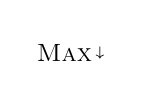
\begin{tikzpicture}[xscale=0.6,yscale=0.4]
\node (max) at (0,0) {{\small \textsc{Max}}};
\node (reg) at (0.75,0.5) {{\fns \textalpha}};
\node (arrow) at (0.75,0) {{\tiny $\downarrow$}};
\node (Rt) at (0.75,-0.5) {{\fns \textbeta}};
\end{tikzpicture}
\end{minipage}
}

\newcommand{\DepAB}{
\begin{minipage}{0.09\textwidth}
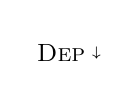
\begin{tikzpicture}[xscale=0.6,yscale=0.4]
\node (max) at (0,0) {{\small \textsc{Dep}}};
\node (reg) at (0.75,0.5) {{\fns \textalpha}};
\node (arrow) at (0.75,0) {{\tiny $\downarrow$}};
\node (Rt) at (0.75,-0.5) {{\fns \textbeta}};
\end{tikzpicture}
\end{minipage}
}

\newcommand{\DepHReg}{
\begin{minipage}{0.055\textwidth}
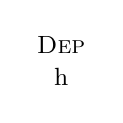
\begin{tikzpicture}[xscale=0.6,yscale=0.4]
\node (dep) at (0,0) {{\small \textsc{Dep}}};
\node (reg) at (0,-1.0) {{\small h}};
\end{tikzpicture}
\end{minipage}
}

\newcommand{\DepLReg}{
\begin{minipage}{0.055\textwidth}
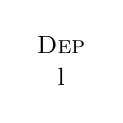
\begin{tikzpicture}[xscale=0.6,yscale=0.4]
\node (dep) at (0,0) {{\small \textsc{Dep}}};
\node (reg) at (0,-1.0) {{\small l}};
\end{tikzpicture}
\end{minipage}
}

\newcommand{\DepReg}{
\begin{minipage}{0.055\textwidth}
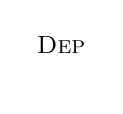
\begin{tikzpicture}[xscale=0.6,yscale=0.4]
\node (dep) at (0,0) {{\small \textsc{Dep}}};
\node (reg) at (0,-1.0) {{\small \textrho}};
\end{tikzpicture}
\end{minipage}
}

\newcommand{\DepTRt}{
\begin{minipage}{0.1\textwidth}
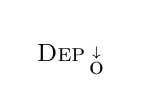
\begin{tikzpicture}[xscale=0.6,yscale=0.4]
\node (dep) at (0,0) {{\small \textsc{Dep}}};
\node (t) at (0.75,0.5) {{\fns \texttau}};
\node (arrow) at (0.75,0) {{\tiny $\downarrow$}};
\node (Rt) at (0.75,-0.5) {{\fns o}};
\end{tikzpicture}
\end{minipage}
}

\newcommand{\MaxRegRt}{
\begin{minipage}{0.1\textwidth}
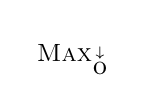
\begin{tikzpicture}[xscale=0.6,yscale=0.4]
\node (max) at (0,0) {{\small \textsc{Max}}};
\node (arrow) at (0.75,0) {{\tiny $\downarrow$}};
\node (Rt) at (0.75,-0.5) {{\fns o}};
\node (reg) at (0.75,0.5) {{\fns \textrho}};
\end{tikzpicture}
\end{minipage}
}

\newcommand{\RegToneByRt}{
\begin{minipage}{0.06\textwidth}
\begin{tikzpicture}[xscale=0.6,yscale=0.5]
\node[rotate=20] (arrow1) at (-0.15,0) {{\fns $\uparrow$}};
\node[rotate=340] (arrow2) at (0.15,0) {{\fns $\uparrow$}};
\node (Rt) at (0,-0.55) {{\small o}};
\node (reg) at (0.4,0.55) {{\small \textrho}};
\node (tone) at (-0.4,0.55) {{\small \texttau}};
\end{tikzpicture}
\end{minipage}
}

\newcommand{\RegToneBySyl}{
\begin{minipage}{0.06\textwidth}
\begin{tikzpicture}[xscale=0.6,yscale=0.5]
\node[rotate=20] (arrow1) at (-0.15,0) {{\fns $\uparrow$}};
\node[rotate=340] (arrow2) at (0.15,0) {{\fns $\uparrow$}};
\node (Rt) at (0,-0.55) {{\small \textsigma}};
\node (reg) at (0.4,0.55) {{\small \textrho}};
\node (tone) at (-0.4,0.55) {{\small \texttau}};
\end{tikzpicture}
\end{minipage}
}

\newcommand{\DepTone}{
\begin{minipage}{0.055\textwidth}
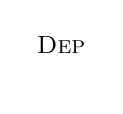
\begin{tikzpicture}[xscale=0.6,yscale=0.4]
\node (dep) at (0,0) {{\small \textsc{Dep}}};
\node (tone) at (0,-1.0) {{\small \texttau}};
\end{tikzpicture}
\end{minipage}
}

\newcommand{\DepTonalRt}{
\begin{minipage}{0.055\textwidth}
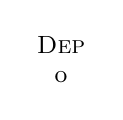
\begin{tikzpicture}[xscale=0.6,yscale=0.4]
\node (dep) at (0,0) {{\small \textsc{Dep}}};
\node (tone) at (0,-1.0) {{\small o}};
\end{tikzpicture}
\end{minipage}
}

\newcommand{\DepL}{
\begin{minipage}{0.055\textwidth}
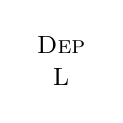
\begin{tikzpicture}[xscale=0.6,yscale=0.4]
\node (dep) at (0,0) {{\small \textsc{Dep}}};
\node (tone) at (0,-1.0) {{\small L}};
\end{tikzpicture}
\end{minipage}
}

\newcommand{\DepH}{
\begin{minipage}{0.055\textwidth}
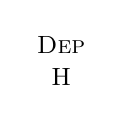
\begin{tikzpicture}[xscale=0.6,yscale=0.4]
\node (dep) at (0,0) {{\small \textsc{Dep}}};
\node (tone) at (0,-1.0) {{\small H}};
\end{tikzpicture}
\end{minipage}
}

\newcommand{\NoMultDiff}{{\small *loh}}
\newcommand{\Alt}{{\small \textsc{Alt}}}
\newcommand{\NoSkip}{{\small \scell{\textsc{No}\\\textsc{Skip}}}}


\newcommand{\RegDomRt}{
\begin{minipage}{0.030\textwidth}
\begin{tikzpicture}[xscale=0.6,yscale=0.5]
\node (arrow) at (0,0) {{\fns $\downarrow$}};
\node (Rt) at (0,-0.55) {{\small o}};
\node (reg) at (0,0.55) {{\small \textrho}};
\end{tikzpicture}
\end{minipage}
}

\newcommand{\DepRegRt}{
\begin{minipage}{0.1\textwidth}
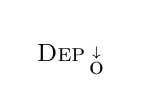
\begin{tikzpicture}[xscale=0.6,yscale=0.4]
\node (dep) at (0,0) {{\small \textsc{Dep}}};
\node (arrow) at (0.75,0) {{\tiny $\downarrow$}};
\node (Rt) at (0.75,-0.5) {{\fns o}};
\node (reg) at (0.75,0.5) {{\fns \textrho}};
\end{tikzpicture}
\end{minipage}
}

% unused

\newcommand{\ToneByRt}{
\begin{minipage}{0.05\textwidth}
\begin{tikzpicture}[xscale=0.6,yscale=0.5]
\node (arrow) at (0,0) {{\fns $\uparrow$}};
\node (Rt) at (0,-0.55) {{\small o}};
\node (tone) at (0,0.55) {{\small \texttau}};
\end{tikzpicture}
\end{minipage}
}

\newcommand{\RegByRt}{
\begin{minipage}{0.05\textwidth}
\begin{tikzpicture}[xscale=0.6,yscale=0.5]
\node (arrow) at (0,0) {{\fns $\uparrow$}};
\node (Rt) at (0,-0.55) {{\small o}};
\node (reg) at (0,0.55) {{\small \textrho}};
\end{tikzpicture}
\end{minipage}
}

\newcommand{\ToneDomRt}{
\begin{minipage}{0.05\textwidth}
\begin{tikzpicture}[xscale=0.6,yscale=0.5]
\node (arrow) at (0,0) {{\fns $\downarrow$}};
\node (Rt) at (0,-0.55) {{\small o}};
\node (tone) at (0,0.55) {{\small \texttau}};
\end{tikzpicture}
\end{minipage}
}

% --- OT tableaus --- %

% Sec. 3.2, first tabl.

\newcommand{\OTHLInput}{
\begin{minipage}{0.17\textwidth}
\begin{tikzpicture}[xscale=\myscalex,yscale=\myscaley]
\node (tone) at (2,0) {(= H)};
\node (syl) at (0,0) {\textsigma};
\node (Rt) at (0,1) {o};
\node (H) at (-0.5,2) {H};
\node (R) at (0.5,3) {h};
\node (Rt2) at (1.5,1.0) {o};
%\node (H2) at (1.0,2) {\epen{L}};
\node (R2) at (2.0,3) {\blue{l}};
\draw [thick] (syl.north) -- (Rt.south) ;
\draw [thick] (Rt.north) -- (H.south) ;
\draw [thick] (Rt.north) -- (R.south) ;
\draw [thick] (syl.north) -- (Rt2.south) ;
%\draw [dashed] (Rt2.north) -- (H2.south) ;
%\draw [dashed] (Rt2.north) -- (R2.south) ;
\end{tikzpicture}
\end{minipage}
}

\newcommand{\OTHLWinner}{
\begin{minipage}{0.17\textwidth}
\begin{tikzpicture}[xscale=\myscalex,yscale=\myscaley]
\node (tone) at (2,0) {(= HL)};
\node (syl) at (0,0) {\textsigma};
\node (Rt) at (0,1) {o};
\node (H) at (-0.5,2) {H};
\node (R) at (0.5,3) {h};
\node (Rt2) at (1.5,1.0) {o};
\node (H2) at (1.0,2) {\epen{L}};
\node (R2) at (2.0,3) {\blue{l}};
\draw [thick] (syl.north) -- (Rt.south) ;
\draw [thick] (Rt.north) -- (H.south) ;
\draw [thick] (Rt.north) -- (R.south) ;
\draw [thick] (syl.north) -- (Rt2.south) ;
\draw [dashed] (Rt2.north) -- (H2.south) ;
\draw [dashed] (Rt2.north) -- (R2.south) ;
\end{tikzpicture}
\end{minipage}
}

\newcommand{\OTHLSpreadingHOnly}{
\begin{minipage}{0.17\textwidth}
\begin{tikzpicture}[xscale=\myscalex,yscale=\myscaley]
\node (tone) at (2,0) {(= HM)};
\node (syl) at (0,0) {\textsigma};
\node (Rt) at (0,1) {o};
\node (H) at (-0.5,2) {H};
\node (R) at (0.5,3) {h};
\node (Rt2) at (1.5,1.0) {o};
%\node (H2) at (1.0,2) {\epen{L}};
\node (R2) at (2.0,3) {\blue{l}};
\draw [thick] (syl.north) -- (Rt.south) ;
\draw [thick] (Rt.north) -- (H.south) ;
\draw [thick] (Rt.north) -- (R.south) ;
\draw [thick] (syl.north) -- (Rt2.south) ;
\draw [dashed] (Rt2.north) -- (R2.south) ;
\draw [dashed] (Rt2.north) -- (H.south) ;
\end{tikzpicture}
\end{minipage}
}

\newcommand{\OTHLInsertH}{
\begin{minipage}{0.17\textwidth}
\begin{tikzpicture}[xscale=\myscalex,yscale=\myscaley]
\node (tone) at (2,0) {(= HM)};
\node (syl) at (0,0) {\textsigma};
\node (Rt) at (0,1) {o};
\node (H) at (-0.5,2) {H};
\node (R) at (0.5,3) {h};
\node (Rt2) at (1.5,1.0) {o};
\node (H2) at (1.0,2) {\epen{H}};
\node (R2) at (2.0,3) {\blue{l}};
\draw [thick] (syl.north) -- (Rt.south) ;
\draw [thick] (Rt.north) -- (H.south) ;
\draw [thick] (Rt.north) -- (R.south) ;
\draw [thick] (syl.north) -- (Rt2.south) ;
\draw [dashed] (Rt2.north) -- (H2.south) ;
\draw [dashed] (Rt2.north) -- (R2.south) ;
\end{tikzpicture}
\end{minipage}
}

\newcommand{\OTHLOverwriting}{
\begin{minipage}{0.17\textwidth}
\begin{tikzpicture}[xscale=\myscalex,yscale=\myscaley]
\node (syl) at (0,0) {\textsigma};
\node (Rt) at (0,1) {o};
\node (H) at (-0.5,2) {H};
\node (R) at (0.5,3) {h};
\node (Rt2) at (1.5,1.0) {o};
%\node (H2) at (1.0,2) {\epen{L}};
\node (R2) at (2.0,3) {\blue{l}};
\draw [thick] (syl.north) -- (Rt.south) ;
\draw [thick] (Rt.north) -- (H.south) ;
\draw [thick] (Rt.north) -- (R.south) ;
\draw [thick] (syl.north) -- (Rt2.south) ;
%\draw [dashed] (Rt2.north) -- (H2.south) ;
\draw [dashed] (Rt.north) -- (R2.south) ;
\node (del) at (0.3,1.9) {\textbf{=}};
\end{tikzpicture}
\end{minipage}
}

\newcommand{\OTHLSpreading}{
\begin{minipage}{0.17\textwidth}
\begin{tikzpicture}[xscale=\myscalex,yscale=\myscaley]
\node (syl) at (0,0) {\textsigma};
\node (Rt) at (0,1) {o};
\node (H) at (-0.5,2) {H};
\node (R) at (0.5,3) {h};
\node (Rt2) at (1.5,1.0) {o};
%\node (H2) at (1.0,2) {\epen{L}};
\node (R2) at (2.0,3) {\blue{l}};
\draw [thick] (syl.north) -- (Rt.south) ;
\draw [thick] (Rt.north) -- (H.south) ;
\draw [thick] (Rt.north) -- (R.south) ;
\draw [thick] (syl.north) -- (Rt2.south) ;
%\draw [dashed] (Rt2.north) -- (H2.south) ;
\draw [dashed] (Rt2.north) -- (H.south) ;
\draw [dashed] (Rt2.north) -- (R.south) ;
\end{tikzpicture}
\end{minipage}
}

% Sec. 4.2, second tabl.: phrase-medial position

\newcommand{\OTHnoLInput}{
\begin{minipage}{0.17\textwidth}
\begin{tikzpicture}[xscale=\myscalex,yscale=\myscaley]
\node (tone) at (2,0) {(= H)};
\node (syl) at (0,0) {\textsigma};
\node (Rt) at (0,1) {o};
\node (H) at (-0.5,2) {H};
\node (R) at (0.5,3) {h};
\node (Rt2) at (1.5,1.0) {o};
%\node (H2) at (1.0,2) {\epen{L}};
%\node (R2) at (2.0,3) {\blue{l}};
\draw [thick] (syl.north) -- (Rt.south) ;
\draw [thick] (Rt.north) -- (H.south) ;
\draw [thick] (Rt.north) -- (R.south) ;
\draw [thick] (syl.north) -- (Rt2.south) ;
\end{tikzpicture}
\end{minipage}
}

\newcommand{\OTHnoLEpenth}{
\begin{minipage}{0.17\textwidth}
\begin{tikzpicture}[xscale=\myscalex,yscale=\myscaley]
\node (tone) at (2,0) {(= HM)};
\node (syl) at (0,0) {\textsigma};
\node (Rt) at (0,1) {o};
\node (H) at (-0.5,2) {H};
\node (R) at (0.5,3) {h};
\node (Rt2) at (1.5,1.0) {o};
\node (H2) at (1.0,2) {\epen{L}};
\node (R2) at (2.0,3) {\epen{h}};
\draw [thick] (syl.north) -- (Rt.south) ;
\draw [thick] (Rt.north) -- (H.south) ;
\draw [thick] (Rt.north) -- (R.south) ;
\draw [thick] (syl.north) -- (Rt2.south) ;
\draw [dashed] (Rt2.north) -- (H2.south) ;
\draw [dashed] (Rt2.north) -- (R2.south) ;
\end{tikzpicture}
\end{minipage}
}

\newcommand{\OTHnoLSpreading}{
\begin{minipage}{0.17\textwidth}
\begin{tikzpicture}[xscale=\myscalex,yscale=\myscaley]
\node (tone) at (2,0) {(= HH)};
\node (syl) at (0,0) {\textsigma};
\node (Rt) at (0,1) {o};
\node (H) at (-0.5,2) {H};
\node (R) at (0.5,3) {h};
\node (Rt2) at (1.5,1.0) {o};
%\node (H2) at (1.0,2) {\epen{L}};
%\node (R2) at (2.0,3) {\blue{l}};
\draw [thick] (syl.north) -- (Rt.south) ;
\draw [thick] (Rt.north) -- (H.south) ;
\draw [thick] (Rt.north) -- (R.south) ;
\draw [thick] (syl.north) -- (Rt2.south) ;
\draw [dashed] (Rt2.north) -- (H.south) ;
\draw [dashed] (Rt2.north) -- (R.south) ;
\end{tikzpicture}
\end{minipage}
}

% Sec. 4.2, third tabl., LM is unaffected by L\%

\newcommand{\OTLMInput}{
\begin{minipage}{0.2\textwidth}
\begin{tikzpicture}[xscale=\myscalex,yscale=\myscaley]
\node (tone) at (2,0) {(= LM)};
\node (syl) at (0,0) {\textsigma};
\node (Rt) at (0,1) {o};
\node (H) at (-0.5,2) {L};
\node (R) at (0.5,3) {l};
\node (Rt2) at (1.5,1.0) {o};
\node (H2) at (1.0,2) {L};
\node (R2) at (2.0,3) {h};
\node (R3) at (3.0,3) {\blue{l}};
\draw [thick] (syl.north) -- (Rt.south) ;
\draw [thick] (Rt.north) -- (H.south) ;
\draw [thick] (Rt.north) -- (R.south) ;
\draw [thick] (syl.north) -- (Rt2.south) ;
\draw [thick] (Rt2.north) -- (H2.south) ;
\draw [thick] (Rt2.north) -- (R2.south) ;
\end{tikzpicture}
\end{minipage}
}

\newcommand{\OTLMReplace}{
\begin{minipage}{0.2\textwidth}
\begin{tikzpicture}[xscale=\myscalex,yscale=\myscaley]
\node (tone) at (2,0) {(= LL)};
\node (syl) at (0,0) {\textsigma};
\node (Rt) at (0,1) {o};
\node (H) at (-0.5,2) {L};
\node (R) at (0.5,3) {l};
\node (Rt2) at (1.5,1.0) {o};
\node (H2) at (1.0,2) {L};
\node (R2) at (2.0,3) {h};
\node (R3) at (3.0,3) {\blue{l}};
\draw [thick] (syl.north) -- (Rt.south) ;
\draw [thick] (Rt.north) -- (H.south) ;
\draw [thick] (Rt.north) -- (R.south) ;
\draw [thick] (syl.north) -- (Rt2.south) ;
\draw [thick] (Rt2.north) -- (H2.south) ;
\draw [thick] (Rt2.north) -- (R2.south) ;
\draw [dashed] (Rt2.north) -- (R3.south) ;
\node (del) at (1.8,2.1) {\textbf{=}};
\end{tikzpicture}
\end{minipage}
}

\newcommand{\OTLMTwoReg}{
\begin{minipage}{0.2\textwidth}
\begin{tikzpicture}[xscale=\myscalex,yscale=\myscaley]
\node (tone) at (2,0) {(= LML)};
\node (syl) at (0,0) {\textsigma};
\node (Rt) at (0,1) {o};
\node (H) at (-0.5,2) {L};
\node (R) at (0.5,3) {l};
\node (Rt2) at (1.5,1.0) {o};
\node (H2) at (1.0,2) {L};
\node (R2) at (2.0,3) {h};
\node (R3) at (3.0,3) {\blue{l}};
\draw [thick] (syl.north) -- (Rt.south) ;
\draw [thick] (Rt.north) -- (H.south) ;
\draw [thick] (Rt.north) -- (R.south) ;
\draw [thick] (syl.north) -- (Rt2.south) ;
\draw [thick] (Rt2.north) -- (H2.south) ;
\draw [thick] (Rt2.north) -- (R2.south) ;
\draw [dashed] (Rt2.north) -- (R3.south) ;
\end{tikzpicture}
\end{minipage}
}

% Sec. 4.2, fourth tabl., L is affected by L\% but M is not

\newcommand{\OTLInput}{
\begin{minipage}{0.17\textwidth}
\begin{tikzpicture}[xscale=\myscalex,yscale=\myscaley]
\node (tone) at (2,0) {(= L)};
\node (syl) at (0,0) {\textsigma};
\node (Rt) at (0,1) {o};
\node (H) at (-0.5,2) {L};
\node (R) at (0.5,3) {l};
\node (R2) at (2,3) {\blue{l}};
\draw [thick] (syl.north) -- (Rt.south) ;
\draw [thick] (Rt.north) -- (H.south) ;
\draw [thick] (Rt.north) -- (R.south) ;
\end{tikzpicture}
\end{minipage}
}

\newcommand{\OTLLowered}{
\begin{minipage}{0.17\textwidth}
\begin{tikzpicture}[xscale=\myscalex,yscale=\myscaley]
\node (tone) at (2,0) {(= LL)};
\node (syl) at (0,0) {\textsigma};
\node (Rt) at (0,1) {o};
\node (H) at (-0.5,2) {L};
\node (R) at (0.5,3) {l};
\node (R2) at (2,3) {\blue{l}};
\draw [thick] (syl.north) -- (Rt.south) ;
\draw [thick] (Rt.north) -- (H.south) ;
\draw [thick] (Rt.north) -- (R.south) ;
\draw [dashed] (Rt.north) -- (R2.south) ;
\end{tikzpicture}
\end{minipage}
}

\newcommand{\OTMInput}{
\begin{minipage}{0.17\textwidth}
\begin{tikzpicture}[xscale=\myscalex,yscale=\myscaley]
\node (tone) at (2,0) {(= M)};
\node (syl) at (0,0) {\textsigma};
\node (Rt) at (0,1) {o};
\node (H) at (-0.5,2) {L};
\node (R) at (0.5,3) {h};
\node (R2) at (2,3) {\blue{l}};
\draw [thick] (syl.north) -- (Rt.south) ;
\draw [thick] (Rt.north) -- (H.south) ;
\draw [thick] (Rt.north) -- (R.south) ;
\end{tikzpicture}
\end{minipage}
}

\newcommand{\OTMLowered}{
\begin{minipage}{0.17\textwidth}
\begin{tikzpicture}[xscale=\myscalex,yscale=\myscaley]
\node (tone) at (2,0) {(= ML)};
\node (syl) at (0,0) {\textsigma};
\node (Rt) at (0,1) {o};
\node (H) at (-0.5,2) {L};
\node (R) at (0.5,3) {h};
\node (R2) at (2,3) {\blue{l}};
\draw [thick] (syl.north) -- (Rt.south) ;
\draw [thick] (Rt.north) -- (H.south) ;
\draw [thick] (Rt.north) -- (R.south) ;
\draw [dashed] (Rt.north) -- (R2.south) ;
\end{tikzpicture}
\end{minipage}
}

% Sec. 4.2, fifth tableau, polar questions with level tones

\newcommand{\OTLPolIn}{
\begin{minipage}{0.20\textwidth}
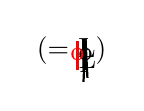
\begin{tikzpicture}[xscale=\myscalex-0.05,yscale=\myscaley-0.05]
\node (tone) at (3.5,0) {(= L)};
\node (syl) at (0,0) {\textsigma};
\node (syl2) at (2,0) {\red{\textsigma}};
\node (Rt) at (0,1) {o};
\node (H) at (-0.5,2) {L};
\node (R) at (0.5,3) {l};
\node (Rt2) at (2,1) {\red{o}};
\draw [thick] (syl.north) -- (Rt.south) ;
\draw [thick,red] (syl2.north) -- (Rt2.south) ;
\draw [thick] (Rt.north) -- (H.south) ;
\draw [thick] (Rt.north) -- (R.south) ;
\end{tikzpicture}
\end{minipage}
}

\newcommand{\OTLPolDef}{
\begin{minipage}{0.20\textwidth}
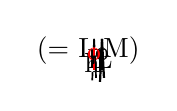
\begin{tikzpicture}[xscale=\myscalex-0.05,yscale=\myscaley-0.05]
\node (tone) at (3.5,0) {(= L.M)};
\node (syl) at (0,0) {\textsigma};
\node (syl2) at (2,0) {\red{\textsigma}};
\node (Rt) at (0,1) {o};
\node (H) at (-0.5,2) {L};
\node (R) at (0.5,3) {l};
\node (H2) at (1.5,2) {\epen{L}};
\node (R2) at (2.5,3) {\epen{h}};
\node (Rt2) at (2,1) {\red{o}};
\draw [thick] (syl.north) -- (Rt.south) ;
\draw [thick,red] (syl2.north) -- (Rt2.south) ;
\draw [thick] (Rt.north) -- (H.south) ;
\draw [thick] (Rt.north) -- (R.south) ;
\draw [semithick,dashed] (Rt2.north) -- (H2.south) ;
\draw [semithick,dashed] (Rt2.north) -- (R2.south) ;
\end{tikzpicture}
\end{minipage}
}

\newcommand{\OTLPolAlt}{
\begin{minipage}{0.20\textwidth}
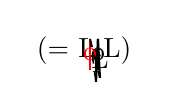
\begin{tikzpicture}[xscale=\myscalex-0.05,yscale=\myscaley-0.05]
\node (tone) at (3.5,0) {(= L.L)};
\node (syl) at (0,0) {\textsigma};
\node (syl2) at (2,0) {\red{\textsigma}};
\node (Rt) at (0,1) {o};
\node (H) at (-0.5,2) {L};
\node (R) at (0.5,3) {l};
\node (Rt2) at (2,1) {\red{o}};
\draw [thick] (syl.north) -- (Rt.south) ;
\draw [thick,red] (syl2.north) -- (Rt2.south) ;
\draw [thick] (Rt.north) -- (H.south) ;
\draw [thick] (Rt.north) -- (R.south) ;
\draw [semithick,dashed] (Rt2.north) -- (H.south) ;
\draw [semithick,dashed] (Rt2.north) -- (R.south) ;
\end{tikzpicture}
\end{minipage}
}

% Sec. 4.2, sixth tableau, polar questions with contour tones

\newcommand{\OTLLPolIn}{
\begin{minipage}{0.23\textwidth}
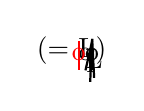
\begin{tikzpicture}[xscale=\myscalex-0.05,yscale=\myscaley-0.05]
\node (tone) at (5.2,0) {(= L)};
\node (syl) at (0,0) {\textsigma};
\node (syl3) at (3.4,0) {\red{\textsigma}};
\node (Rt) at (0,1) {o};
\node (Rt2) at (1.7,1) {o};
\node (Rt3) at (3.4,1) {\red{o}};
\node (H) at (-0.5,2) {L};
\node (R) at (0.5,3) {l};
\draw [thick] (syl.north) -- (Rt.south) ;
\draw [thick] (syl.north) -- (Rt2.south) ;
\draw [thick,red] (syl3.north) -- (Rt3.south) ;
\draw [thick] (Rt.north) -- (H.south) ;
\draw [thick] (Rt.north) -- (R.south) ;
\end{tikzpicture}
\end{minipage}
}

\newcommand{\OTLLPolDef}{
\begin{minipage}{0.23\textwidth}
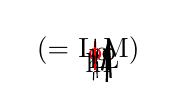
\begin{tikzpicture}[xscale=\myscalex-0.05,yscale=\myscaley-0.05]
\node (tone) at (5.2,0) {(= L.M)};
\node (syl) at (0,0) {\textsigma};
\node (syl3) at (3.4,0) {\red{\textsigma}};
\node (Rt) at (0,1) {o};
\node (Rt2) at (1.7,1) {o};
\node (Rt3) at (3.4,1) {\red{o}};
\node (H) at (-0.5,2) {L};
\node (R) at (0.5,3) {l};
\node (H3) at (2.9,2) {\epen{L}};
\node (R3) at (3.9,3) {\epen{h}};
\draw [thick] (syl.north) -- (Rt.south) ;
\draw [thick] (syl.north) -- (Rt2.south) ;
\draw [thick,red] (syl3.north) -- (Rt3.south) ;
\draw [thick] (Rt.north) -- (H.south) ;
\draw [thick] (Rt.north) -- (R.south) ;
\draw [dashed] (Rt3.north) -- (H3.south) ;
\draw [dashed] (Rt3.north) -- (R3.south) ;
\end{tikzpicture}
\end{minipage}
}

\newcommand{\OTLLPolSkip}{
\begin{minipage}{0.23\textwidth}
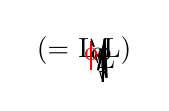
\begin{tikzpicture}[xscale=\myscalex-0.05,yscale=\myscaley-0.05]
\node (tone) at (5.2,0) {(= L.L)};
\node (syl) at (0,0) {\textsigma};
\node (syl3) at (3.4,0) {\red{\textsigma}};
\node (Rt) at (0,1) {o};
\node (Rt2) at (1.7,1) {o};
\node (Rt3) at (3.4,1) {\red{o}};
\node (H) at (-0.5,2) {L};
\node (R) at (0.5,3) {l};
\draw [thick] (syl.north) -- (Rt.south) ;
\draw [thick] (syl.north) -- (Rt2.south) ;
\draw [thick,red] (syl3.north) -- (Rt3.south) ;
\draw [thick] (Rt.north) -- (H.south) ;
\draw [thick] (Rt.north) -- (R.south) ;
\draw [dashed] (Rt3.north) -- (H.south) ;
\draw [dashed] (Rt3.north) -- (R.south) ;
\end{tikzpicture}
\end{minipage}
}  
  
\newcommand{\ilit}[1]{#1\il{#1}}    
\newcommand{\isit}[1]{#1\is{#1}}  

\makeatletter
\let\thetitle\@title
\let\theauthor\@author 
\makeatother

\newcommand{\togglepaper}[1][0]{ 
  \bibliography{../localbibliography}
  %% hyphenation points for line breaks
%% Normally, automatic hyphenation in LaTeX is very good
%% If a word is mis-hyphenated, add it to this file
%%
%% add information to TeX file before \begin{document} with:
%% %% hyphenation points for line breaks
%% Normally, automatic hyphenation in LaTeX is very good
%% If a word is mis-hyphenated, add it to this file
%%
%% add information to TeX file before \begin{document} with:
%% \include{localhyphenation}
\hyphenation{
affri-ca-te
affri-ca-tes
com-ple-ments
par-a-digm
Sha-ron
Kings-ton
phe-nom-e-non
Daul-ton
Abu-ba-ka-ri
Ngo-nya-ni
Clem-ents 
King-ston
Tru-cken-brodt
Tab-leau
cophono-logies
mark-edness
Ti-gri-nya
a-mong
Car-stens
Lu-bu-ku-su
}
\hyphenation{
affri-ca-te
affri-ca-tes
com-ple-ments
par-a-digm
Sha-ron
Kings-ton
phe-nom-e-non
Daul-ton
Abu-ba-ka-ri
Ngo-nya-ni
Clem-ents 
King-ston
Tru-cken-brodt
Tab-leau
cophono-logies
mark-edness
Ti-gri-nya
a-mong
Car-stens
Lu-bu-ku-su
}
  \papernote{\scriptsize\normalfont
    \theauthor.
    \thetitle. 
    To appear in: 
    Emily Clem,   Peter Jenks \& Hannah Sande.
    Theory and description in African Linguistics: Selected papers from the 47th Annual Conference on African Linguistics.
    Berlin: Language Science Press. [preliminary page numbering]
  }
  \pagenumbering{roman}
  \setcounter{chapter}{#1}
  \addtocounter{chapter}{-1}
}

\newcommand{\upstep}{\textupstep}


% \newcounter{tableauxcounter}

\renewcommand{\textltailn}{ɲ}
\renewcommand{\textbardotlessj}{ɟ}

\newcommand{\emphkh}[1]{\textit{#1}} %originally \textbf, banned by the guidelines



\definecolor{lsDOIGray}{cmyk}{0,0,0,0.45}


\newcommand{\xuparrow}[1]{%
  {\left\uparrow\vbox to #1{}\right.\kern-\nulldelimiterspace}
}
\renewcommand \textupstep[1]{\char"A71B#1}
\renewcommand \textdownstep[1]{\char"A71C#1}
 
 \newcommand{\ꜛ}{\textsf{ꜛ}}
 
\def\biberror{\undefined}


\newcommand{\OTbox}[1]{\resizebox{.88\textwidth}{!}{#1}}


\title{Stem modification in Nuer}
\author{Irina Monich\affiliation{University of Surrey} \lastand  Matthew Baerman\affiliation{University of Surrey}}


\abstract{Nuer is a Western Nilotic language remarkably rich in non-concatenative morphology.  This article provides a comprehensive description of those morphological processes in Nuer that are responsible for variations in the form of the stem.  Our data shows that all stem-modifying operations have one of the following four targets in the stem: stem vowel quality and quantity, tonal melody, and properties of the stem-final consonant.  The vowel quality modification is comprised of two separate processes where either lowering and removal of breathiness is applied or raising and addition of breathiness. Thus vowel quality modification yields two separate series of mutated vowels.  We provide arguments for treating some vowels as basic, while others as derived.  We also identify tonal patterns found in verbal morphology, and three types of morphologically triggered consonantal lenition.  According to our findings, exactly the same processes apply in both the nominal and the verbal system.}

\begin{document}

\maketitle

\section{Introduction} %1. /

\ili{Nuer} is a Western \ili{Nilotic} language of the \ili{Nilo-Saharan} language family with almost 900,000 speakers worldwide.  It is part of \ili{Dinka}-\ili{Nuer} language cluster which also includes \ili{Thok Reel}. 

\ili{Nuer} has attracted attention for the complexity of its nominal inflection, which employs a baffling variety of forms in a seemingly chaotic lexical and paradigmatic distribution \citep{Frank1999, Baerman2012}. \tabref{tab:monich:1} offers a taste of this, showing a small sample of the various schemes of affixation and \isi{stem modification} displayed by different nouns. (All examples in this paper come from our own fieldwork.)


\begin{table}
\begin{tabularx}{\textwidth}{XXlXlX}
\lsptoprule
\bfseries\scshape nom sg & \bfseries\scshape gen sg & \bfseries\scshape loc sg & \bfseries\scshape nom pl & \bfseries\scshape gen/loc pl & \bfseries Gloss\\
\midrule
kɛɛɛt & \multicolumn{2}{c}{kɛɛɛt-ʌ̤} & \multicolumn{2}{c}{kɛɛɛt-ní} & ‘stick’\\
têr̥ & \multicolumn{2}{c}{té̤r̥-ʌ̤} & té̤r̥ & têeet & ‘hand’\\
kɔ̤aaaɣ & kɔ̤ah & kɔ̤h & kɔ̤aɣ & kɔ̤aaɣ-nì & ‘hole’\\
kíir & kîɛɛɛr & kîiir & kîɛr & kîɛr-ì & ‘big river’\\
\lspbottomrule
\end{tabularx}
\caption{A sample set of nominal paradigms (Western variety, Bentiu)}
\label{tab:monich:1}
\end{table}

An obvious requirement for understanding this system is to isolate the morphological devices involved, no mean feat given its high degree of lexical idiosyncrasy. In this paper we set out to do this, focusing on the system (or systems) of \isi{stem modification}. The key to this lies in \isi{verbal morphology}, which employs the same devices found in nominal inflection – manipulation of quality, quantity and \isi{tone} of the stem vowel and manner of articulation of the stem-final consonant – but with a high degree of regularity and predictability. Further, by doing this we can show that there are two distinct kinds of \isi{vowel quality} modifying processes. One is primarily a lowering process, and is associated with case-number inflection in nouns and person-number inflection in verbs. The other involves vowel raising, and is associated with number inflection in nouns and derivation in verbs.

Language consultants used for this study are all native speakers of \ili{Nuer}.  Of the ten consultants four are representative of the Western variety of \ili{Nuer} (Bentiu), and the other six are speakers of the Eastern dialect of \ili{Nuer} (\ili{Jikany}\footnote{One of our \ili{Jikany} \ili{Nuer} consultants spent his formative years in Akobo area of South Sudan; the other five  originate from Nasir.  The variety of \ili{Nuer} spoken by the Akobo native does not appear to be different from that spoken by other \ili{Jikany} \ili{Nuer} consultants.  By contrast, differences between the Eastern (\ili{Jikany}) and Western (Bentiu) dialects are clearly defined in several areas of grammar.  Therefore, we indicate throughout this article whether data comes from Eastern or Western variety of \ili{Nuer}, without drawing further dialectal distinctions.}).  All currently reside outside of South Sudan (UK and USA) but use \ili{Nuer} on a daily basis within their communities.  

The major prior source on \ili{Nuer} is \citet{Crazzolara1933}. Other notable previous works include \citet{Vandevortnd}'s draft pedagogical grammar, and \citet{Frank1999} and \citet{Storch2005} on noun morphology.  The transcription of data in these sources is often inconsistent, especially in regards to the subtle contrasts of \isi{vowel quality} and \isi{tone}.  Since much of morphological contrasts in \ili{Nuer} are signaled by manipulation of precisely these properties, errors in data transcription make it difficult to arrive at phonological operations that are at the heart of \ili{Nuer} morphology.  Before we can truly evaluate the complexity of \ili{Nuer} verbal and nominal systems, it is essential to establish the basic phonological alternations that play such an important role in \ili{Nuer} grammar.

More recent work on \ili{Nuer} includes
\citeauthor{gjersøe2016} (\citeyear{gjersøe2016}; \citeyear{gjersøe2017}) on \isi{tone}, Reid (forthcoming) on \isi{verbal morphology}, \citet{Faust2017} on vowel alternations in adjectival reduplication, and \citet{faust2015} which provides general overview of the grammar of a \ili{Jikany} variety from Nasir. Some of the findings reported here contradict or overlap with the findings in these works.  The vowel correspondences are generally aligned with the ones identified by \citet{Faust2017} and \citet{faust2015} but with some important differences mainly involving documentation of breathiness and diphthongization.  The tonal inventory that we identify here is richer than the one proposed in \citeauthor{gjersøe2016} (\citeyear{gjersøe2016}; \citeyear{gjersøe2017}), and it allows for more precise classification of tonal patterns.  Where applicable, important differences between these works and ours will be pointed out throughout this article.

\section{Basics of Nuer phonology} %2. /

Both varieties of \ili{Nuer} discussed here distinguish (at least) fifteen vowel phonemes, shown in \figref{fig:monich:1}a.  Most of these constitute part of a modal/breathy pair (breathiness is indicated by two dots underneath the first grapheme of a vowel).  Except for the high mid range, the breathy counterpart is typically somewhat higher in the vowel space. There are also four pairs of modal/breathy diphthongs (\figref{fig:monich:1}b). 


%\begin{figure}
%\begin{tabular}{ccccccc}
%i i & & & & & & u ṳ	\\
%&	e e	& & & & o o	\\
%& &	ɛ ɛ & & ɔ ɔ	\\
%& & & ʌ	\\
%& & & a a	\\
%\end{tabular}
%\begin{tabular}{ccccccc}
%iɛ ie & & & & & & uɔ ṳo	\\
%&\\
%& & ɛa ɛ a & & ɔa ɔ a	\\
%&\\
%&\\	
%\end{tabular}
%\label{fig:monich:1}
%\caption{Nuer vowel inventory}
%\end{figure}

\begin{figure}
	\includegraphics[width=\textwidth]{figures/fig-monich-1.png}
	\caption{Nuer vowel inventory}
	\label{fig:monich:1}
\end{figure}


Even though the vowels listed in Fig 1 are all contrastive in \ili{Nuer}, we argue here that they do not all have equal status in \ili{Nuer} grammar.  Only vowels /a, ɔ, ɔ̤, ɛ ɛ̤, i and u/ are found in the morphologically “basic” form of the root.  All diphthongs, as well as monophthongs /a̤, ʌ̤, e, e̤, o, o̤, i̤ and ṳ/, emerge as a result of morphological modification of the stem.  These vowels are produced when affixes consisting of floating features superimpose on the vowel of the stem, modifying its properties.  Consequently, they signal morphological rather than lexical contrasts.

Both diphthongs and monophthongs occur in three degrees of length: short, long and overlong, represented here by three vowel graphemes, plus onglide in the case of diphthongs. Breathiness is indicated on the first grapheme alone. There are two lexically specified tones:  H and L.  Rising and falling tones also occur but their appearance is either phonologically conditioned or results from combination of H and L tones.  Falling and high tones are neutralized depending on the phonation of the vowel: if the vowel is breathy, the falling and high tones are both realized as high, while over modal vowels the two tones are both realized as falling.  Rising tones emerge as a result of fissure of spread H-tones into L and H (also applies to adjacent H-tones in the same word).  In other words, there is a rule HH $\rightarrow$ LH that takes place word-internally\footnote{Full justification for positing this rule cannot be offered here due to space limitations.  One supporting piece of evidence is that before high-toned suffixes, the \isi{tone} over a short intransitive stem can only be L or LH. At the same time, before low-toned suffixes, the \isi{tone} of the stem may be either high or low.  This state of affairs can be accounted for assuming that short roots are lexically specified as L or H, and that this lexical tones appear as such before low-toned suffixes.  However, before H-toned suffixes the H of the stem breaks into L and H.  Such analysis also allows for a better understanding of derivation of tonal melodies in transitive stems in \sectref{sec:monich:3.3}}. As with breathiness, \isi{tone} is indicated on the first grapheme of a multi-graphemic vowel representation.

The consonantal inventory of \ili{Nuer} is shown in \tabref{tab:monich:2}.  In intervocalic position the stem-final consonants tend to become voiced.  The phonemes in parenthesis are only contrastive in stem-final position in some varieties of Western \ili{Nuer}.


\begin{table}
\begin{tabularx}{\textwidth}{XXXXXX}
\lsptoprule
& \bfseries Labial & \bfseries Dental & \bfseries Alveolar & \bfseries Palatal & \bfseries Velar\\
\midrule 
Voiceless stops & p & t̪ & t & c & k\\
Voiced stops & b & d̪ & d & ɟ & g\\
Fricative & (f) & (θ) & (r̥) & (ç) & (h)\\
Nasal & m & n̪ & n & ɲ & ŋ\\
Lateral &  &  & l &  & \\
Trill &  &  & r &  & \\
Glides & w &  &  & j & ɣ\\
\lspbottomrule
\end{tabularx}
\caption{Consonantal phonemes}
\label{tab:monich:2}
\end{table}

\section{Verbal inflection}
\subsection{Overview} %3.1 /

We \isi{focus} here on inflection for \isi{subject} person-number, which occurs in the Present Imperfect Positive Tense when used with a preverbal \isi{subject}.  A sample paradigm is provided in \tabref{tab:monich:3}, including other forms which we will discuss below only in passing.

\begin{table}
\begin{tabularx}{\textwidth}{llrll}
\lsptoprule
 & \bfseries Singular & \multicolumn{2}{c}{\bfseries Plural} & \bfseries Other forms\\
\midrule
1  & pɔ̤́aaad-ʌ̤̀ & \multicolumn{1}{r}{pɔ̤̌ar̥-kɔ̤̌ (\textsc{excl})} & \multicolumn{1}{l}{pɔ̤̌ar̥-nɛ (\textsc{incl})} & NF1 pɔ̤r̥\\
2 & pɔ̤́ɔɔd-ì̤ & \multicolumn{2}{c}{pɔ̤̌ar̥-ɛ} & NF2 pɔ̤t\\
3 & pɔ̤́ɔɔd-ɛ̀ & \multicolumn{2}{c}{pɔ̤̌ar̥-kɛ} & NSF pɔ̤t\\
\lspbottomrule
\end{tabularx}
\caption{‘beat (the drum)\textsc{.tr}’ (Western Nuer)}
\label{tab:monich:3}
\end{table}

NF1 = non-finite form used with \isi{perfect} auxiliaries

NF2 = non-finite form used with non-\isi{perfect} auxiliaries

NSF = non-suffixed form used with a post-verbal suffix\\ 

Besides bearing different inflectional suffixes, the individual forms are distinguished by various stem alternations,\footnote{The term “stem” is used here to label the portion of the word with the exclusion of inflectional suffixes.  Since there are no segmental derivational suffixes, the stem incorporates all derivational morphology.} involving length, \isi{vowel quality}, \isi{tone} and the stem-final consonant.  In the next several sections we review these processes in turn. 

\subsection{Vowel quality modification} %3.2 /

The system of \isi{vowel quality} modification involves a two-way contrast which we designate here as grade 1 vs. 2 and grade A vs. B (\tabref{tab:monich:4}). The system of vowel grades adopted here is almost identical to the one presented by \citet{reid2016} with an important distinction that it is entirely based on the pattern of morphological distribution of the grades, rather than their phonological properties.

\begin{table}
\begin{tabularx}{\textwidth}{XXXX}
\lsptoprule

\multicolumn{2}{c}{  Grade 1} & \multicolumn{2}{c}{  Grade 2}\\
\midrule
  Grade A &  Grade B &  Grade A &  Grade B\\
 i & iɛ & i̤ & i̤e\\
 ɛ & ɛa & e̤ & e\\
 ɛ̤ & ɛ̤a & ɛ̤ & ɛ̤a\\
 a & a & ʌ̤ & a̤\\
 ɔ & ɔa & o̤ & o\\
 ɔ̤ & ɔ̤a & ɔ̤ & ɔ̤a\\
 u & uɔ & ṳ & ṳo\\
\lspbottomrule
\end{tabularx}
\caption{Morphological stem vowel grades in Nuer}
\label{tab:monich:4}
\end{table}

The grades \textit{roughly} correspond to phonological contrasts.  Thus most Grade 1 vowels are modal, while most Grade 2 vowels are breathy, and raised with respect to their Grade 1 counterparts.  The Grade A{\textasciitilde}B alternation for most vowels involves lowering which, wherever possible, yields an opening diphthong; however, in case of the Grade A vowels /e̤/ and /o̤/ we see instead the removal of breathiness to yield Grade B. \footnote{\citet{Faust2017} offers a similar model of inflectional vowel mutation (i.e. derivation of set B from set A in our terms) based on the pattern observed in adjectives, but with two important differences.  First, he does not transcribe the diphthong /ɛa/ (which may be valid for his consultant’s dialect), positing that the modified counterpart of /ɛ/ is /a/.  Most importantly, Faust’s does not distinguish various phonation properties in his transcription.  As a result, in his model, close mid vowels /e/ and /o/ have no modified counterparts.}  

The two sets of alternations have a clear division of labor in the verbal system. Grade 1 vowels are found in underived transitive verbs, while Grade 2 vowels are found with all verbs derived from them. The Grade A {\textasciitilde} B alternation takes place \textit{within} the paradigms of individual verbal lexemes, e.g. between different \isi{subject} person-number values. The distribution of grade A and B differs depending on whether the verb is transitive or intransitive: grade A is used in 2/3\textsc{sg} of all verbs, and additionally in 3\textsc{pl} of intransitive verbs, while grade B is used elsewhere.\footnote{This excludes a relatively small class of intransitive verbs which denote involuntary and reflexive actions and states, such as “get tired”, “cough”, “boil”, “float”, “be alive”, “wash oneself”, etc. These verbs have vowels of grade 2 in all forms, including the non-suffixed forms. \label{fn:monich:5} }  The basic template of the two \isi{vowel quality} modification types is illustrated in \tabref{tab:monich:5} and exemplified in \tabref{tab:monich:6}. 

%\begin{table}
%a. Underived transitive verb b. Derived intransitive (antipassive) verb 
%\begin{tabular}{\textwidth}{XXXXXXX} & \multicolumn{1}{c}{ singular} 
%\hline
%& plural &  &  & \multicolumn{1}{c}{ singular} & plural\\
% 1 &  & Grade 1B &  & 1 &  & Grade 2B\\
% 2 & Grade 1A &  &  & 2 & Grade 2A & \\
%%\hhline{--~----}
%\multicolumn{1}{c}{ 3} &  &  &  & \multicolumn{1}{c}{ 3} &  & \\
%%\hhline{-~~--~-}
%\hline
%\end{tabular}
%\caption{Patterns of vowel quality modification}
%\label{tab:5}
%\end{table}


%TODO Ask if this is the right caption for table 5??
\begin{table}[!htb]
	\begin{subtable}{0.4\linewidth}
	\caption{Transitive verb}
	\begin{tabular}{|ccc|}
		\hline
		& singular & plural\\
		1 & &\\\cline{1-2}
		2 & \multirow{2}{*}{Grade A} & \multicolumn{1}{|c|}{Grade B}\\ 
		3 & &\multicolumn{1}{|c|}{}\\
		\hline
	\end{tabular}
	\end{subtable}
	\begin{subtable}{0.4\linewidth}
	\caption{Intransitive verb}
	\begin{tabular}{|ccc|}
		\hline
		& singular & plural\\
		1 & &\\\cline{1-2}
		2 & \multirow{2}{*}{Grade A} & \multicolumn{1}{|c|}{Grade B}\\\cline{3-3} 
		3 & &\multicolumn{1}{c|}{}\\
		\hline
	\end{tabular}
	\end{subtable}
\caption{a. Underived transitive verb ‘see’ b. Derived intransitive (antipassive) verb ‘see’}
\label{tab:monich:5}
\end{table}

 
\begin{table}
\begin{tabularx}{\textwidth}{lXXXlXX}
\lsptoprule
 & singular & plural &  &  & singular & plural\\
\midrule
 1 & nɛaaanʌ̤ & nɛankɔ &  & 1 & něnʌ̤ & něnkɔ\\
 2 & nɛɛɛnì̤ & nɛanɛ &  & 2 & ne̤ní̤ & něnɛ\\
 3 & nɛɛɛnɛ & nɛankɛ &  & 3 & ne̤nɛ & ně̤nkɛ\\
\lspbottomrule
\end{tabularx}
\caption{Exemplification of the patterns in \tabref{tab:monich:5}}
\label{tab:monich:6}
\end{table}

The motivation for treating the Grade 1A as the “basic” grade from which all others can be derived, will be given in \sectref{sec:monich:6}, after the distribution of vowel grades in the nominal and \isi{verbal morphology} of \ili{Nuer} has been fully described.

\subsection{Other types of stem modification} %3.3 /
\label{sec:monich:3.3}

Variations in vowel quantity, \isi{tone} and properties of the stem-final consonant are also involved in inflectional morphology.  Within the finite paradigm they oppose singular and plural forms, and thus cross-cut the \isi{vowel quality} alternations described above.  Typically only underived transitive verbs are affected.  We divide these into two classes, relevant both for \isi{tone} and vowel quantity alternations. 

Let us first look at \isi{tone}.\footnote{The treatment of \isi{tone} in the verbal system presented in Sections 3 and 4 differs significantly from \citet{gjersøe2017} who reports only two tonal contours in verbs, and does not distinguish contrast between low and rising tones.} Class I verbs have a rising contour in the singular, followed by a high \isi{tone} of the suffix (falling if the vowel of the suffix is modal), and low stem with a low suffix in the plural.\footnote{The \isi{tone} of the 1P\textsc{l} Inclusive form will be ignored throughout the discussion, since it has the same tonal contour for all verbs H-H (realized as LH-HL).} Class II verbs have a falling \isi{tone} (if the stem vowel is modal) or high (if the stem vowel is breathy) \isi{tone} on the stem followed by the low \isi{tone} on the suffix in singular forms, and a rise on the stem followed by the fall on the suffix in plural forms. These patterns are summarized in \tabref{tab:monich:7}, abstracting away from the differences in realization of high and falling tones due to the vowel phonation properties.  The longer singular stem is represented as having two tonal elements (a spread H-\isi{tone} in case of Class I, shown as HH, and an HL in case of Class II), while the short plural stem has a single tonal element.  The \isi{tone} of the inflectional suffix is always the same as the last tonal element of the stem and is therefore presumed to be a result of tonal spreading from the stem. All spread H-tones split into L and H resulting in rising tones (see fn. 2).  

\begin{table}
\begin{tabularx}{\textwidth}{lllXXX}
\lsptoprule
 & Singular & Plural & \multicolumn{2}{c}{Example} & Gloss\\
\midrule
&  &  & \scshape 2sg & \multicolumn{1}{c}{\scshape 2pl} & \\
Class I & HH-H $\rightarrow$ LH-H & L-L & bṳ̌uulí̤ & bɔ̤lɛ & ‘roast’\\
Class II & HL-L & H-H $\rightarrow$ LH-H & nɛɛɛnì̤ & nɛanɛ & ‘see’\\
\lspbottomrule
\end{tabularx}
\caption{Tonal patterns in underived transitive verbs}
\label{tab:monich:7}
\end{table}

Without going into the details of tonal derivation, it deserves mentioning that the tonal values of the plural stem (L for Class I and H for Class II) are the same as the first tonal element of the singular stem. We can propose, therefore, that derivation of the plural stem from the singular stem is accompanied by deletion of the second tonal element in addition to shortening.

With stem length, Class I verbs show some variation across dialects.  In Eastern varieties, they have a short vowel throughout the paradigm.  In Western dialects, stems that end in a sonorant have an overlong vowel in the singular.  Class II verbs (\tabref{tab:monich:9}) are always overlong with singular persons and short with plural persons, in both Eastern and Western dialects. 

\begin{table}
\begin{tabularx}{\textwidth}{lXXXX} 
\lsptoprule
& \multicolumn{2}{c}{Singular} & \multicolumn{2}{c}{Plural}\\
\midrule
& Western \ili{Nuer} & \multicolumn{1}{c}{Eastern Nuer} &  & \\
1 & bɔ̤ɔɔlʌ̤ & bɔ̤lʌ̤ & \multicolumn{1}{c}{bɔ̤lkɔ (\textsc{Excl})} & bɔ̤lnɛ (\textsc{Incl})\\
2 & bṳ̌uulí̤ & bṳ̌lí̤ & \multicolumn{2}{c}{bɔ̤lɛ}\\
3 & bṳ̌uulɛ & bṳ̌lɛ & \multicolumn{2}{c}{bɔ̤lkɛ}\\
\lspbottomrule
\end{tabularx}
\caption{Inflected paradigm of bṳl ‘roast.\textsc{tr}’ (Class I)}
\label{tab:monich:8}
\end{table}


\begin{table}
\begin{tabularx}{\textwidth}{XXXX} 
\lsptoprule
& Singular & \multicolumn{2}{c}{Plural}\\
\midrule
1 & nɛ̂aaanʌ̤̀ & \multicolumn{1}{c}{nɛankɔ (\textsc{Excl})} & nɛanɛ (\textsc{Incl})\\
2 & nɛ̂ɛɛnì̤ & \multicolumn{2}{c}{nɛanɛ}\\
3 & nɛ̂ɛɛnɛ̀ & \multicolumn{2}{c}{nɛankɛ}\\
\lspbottomrule
\end{tabularx}
\caption{Inflected paradigm of nɛɛɛn ‘see.\textsc{tr}’ (Class II)}
\label{tab:monich:9}
\end{table}

One possible interpretation of the East{\textasciitilde}West contrast in Class I is that singular stems in \textit{both} tonal classes have overlong vowels, but that stems that carry rising \isi{tone} (i.e. Class I) undergo shortening.  This can be considered a purely phonological process that applies uniformly in Eastern varieties, but fails to apply in sonorant-final stems in Western varieties.  For the sake of comparison, \tabref{tab:monich:10} shows a Western \ili{Nuer} paradigm of a Class I transitive verb which ends in a non-sonorant.  In contrast to sonorant-final verbs, the stem in \tabref{tab:monich:10} is short in singular forms.  The corresponding Eastern \ili{Nuer} paradigm of this verb is exactly the same, except for the lack of consonantal mutation in the plural.

\begin{table}
\begin{tabularx}{\textwidth}{XXXX} 
\lsptoprule
& Singular & \multicolumn{2}{c}{Plural}\\
\midrule
1 & kɔaɣʌ̤ & \multicolumn{1}{c}{kɔàkɔ (\textsc{Excl})} & kɔahnɛ (\textsc{Incl})\\
2 & kɔɣí̤ & \multicolumn{2}{c}{kɔàhɛ}\\
3 & kɔɣɛ & \multicolumn{2}{c}{kɔàkɛ}\\
\lspbottomrule
\end{tabularx}
\caption{Inflected paradigm of  kɔk ‘buy.\textsc{tr}’ (Class I) (Western Nuer)}
\label{tab:monich:10}
\end{table}

Finally, in Western dialects of \ili{Nuer}, stem-final stops are lenited in the plural (\tabref{tab:monich:11}).  The labial stop /b/ is mutated into /f/,  the interdental stop /t̪/ is mutated into /θ/, and the alveolar stop /d/ becomes a continuant /r̥/. Velar and palatal stops are a special case. The modified variants of /k, g/ and /c, ɟ/ are /h/ and /ҫ/, respectively. However, these stem-final stops themselves undergo a separate process of \isi{lenition} when they are intervocalic: /k, g/ $\rightarrow$ /ɣ/ and /c, ɟ/ $\rightarrow$ /j/.\footnote{Note that this must be understood as a morphophonological process targeting stem consonants, because unlenited intervocalic velars occur in other contexts, e.g. in suffix-initial position. Moreover, the variants [ɣ] and [j] also occur word-finally in nominal forms which contain a lengthened vowel, further supporting the notion that we are dealing with two separate morphophonological \isi{lenition} processes: one that mutates all stops into voiceless continuants, and another that mutates the palatal and velar stops only, yielding voiced continuants.} The result is an alternation between two different continuants. (The underlying stop may be found in other parts of the paradigm; e.g. the NSF of ‘buy\textsc{.tr}’ (the form used with an immediately post-verbal \isi{subject}) is \textit{kɔk}, and the NSF of ‘cane\textsc{.tr}’ is \textit{dwác.})  

 %%please move \begin{table} just above \begin{tabular
\begin{table}
\begin{tabularx}{\textwidth}{XXXXX} 
\lsptoprule
& ‘wait.\textsc{tr}’ & ‘sing.\textsc{tr}’ & ‘buy.\textsc{tr}’ & ‘cane.\textsc{tr}’\\
\midrule
3sg & lîiib-ɛ̀ & kîiid-ɛ̀ & kɔɣ-ɛ & dwʌ̤j-ɛ\\
2pl & lǐɛf-ɛ & kǐɛr̥-ɛ & kɔàh-ɛ & dwǎ̤ç-ɛ\\
\lspbottomrule
\end{tabularx}
\caption{Stem-final consonant lenition (Western Nuer varieties only)}
\label{tab:monich:11}
\end{table}

It is tempting to link the morphologically conditioned consonantal mutation to changes in stem \isi{vowel length}, as was suggested above in regards to tonal alternations. However, consonantal \isi{lenition} also takes place in NF1 forms of all underived transitive verbs but not in NF2 or NSF forms; compare the three forms of ‘wait’: NF1 \textit{lîf}, NF2 \textit{lîb}, NSF \textit{líb}.  Since all three forms are short and have unmodified vowel (in underived transitive verbs), \isi{lenition} of the stem-final consonant so far seems to apply independently from other stem modifying processes.

\section{Verbal derivation} %4. /

Verbal derivation involves \isi{stem modification} alone; there are no derivational affixes. The system is oriented around transitive verbs: as far as we know, all transitive verbs can form a derived intransitive (the antipassive), while all intransitives have the morphological characteristics of derived verbs, whether or not there is a corresponding  underived transitive.  In addition, we have identified derived ditransitive, centripetal and multiplicative paradigms.

All derived verbs have grade 2 stem vowels.\footnote{With the exception of the class of intransitives mentioned in fn. \ref{fn:monich:5}.}  \tabref{tab:monich:12} illustrates the correspondence between basic transitive verbs with grade A stem vowels and derived verbs with grade 2 vowels; note that intransitive ‘fight’ has a grade 2 vowel, even though there is no transitive counterpart.

\begin{table}
\begin{tabularx}{\textwidth}{lXlX}
\lsptoprule
\multicolumn{2}{c}{\bfseries Basic, 2\textsc{sg} (Grade 1)} & \multicolumn{2}{c}{\bfseries Derived, 2\textsc{sg} (Grade 2)}\\
\midrule
t̪âaaɣ{}-ì̤ & ‘hold’ & t̪ʌ̤h-ì̤ & ‘hold for (ditransitive)’\\
ríŋ-ì̤ & ‘run’ & rí̤ŋ-ì̤ & ‘run (centripetal)’\\
cɔɔɔl-ì̤ & ‘call’ & có̤l-i̤ & ‘call for (benefactive)’\\
pṳdi̤ & ‘break’ (once) & pṳr̥-í & ‘break (multiplicative)’\\
nɛɛɛn-ì̤ & ‘see’ (transitive) & ne̤n-í̤ & ‘see (antipassive)’\\
\multicolumn{2}{c}{n/a} & ɲe̤ɲ-ì̤ & ‘fight’ (intransitive)\\
\lspbottomrule
\end{tabularx}
\caption{Vowel quality modification in derived forms (Western Nuer)}
\label{tab:monich:12}
\end{table}

What distinguishes the different types of derived verbs, is their length and tonal properties. We will \isi{focus} here on the antipassives, as these are the most productive and hence best represented in our data.  We distinguish types of antipassives.  Antipassive I involves complete deletion of the \isi{direct object}, while Antipassive II allows the inclusion of a demoted \isi{direct object} with the preposition \textit{kɛ;} compare \textit{mâad̪ì̤} \textit{pi̤u} ‘you are drinking water’ with Antipassive II \textit{mʌ̤d̪ì̤} \textit{kɛ pi̤u} (same translation). 

The two types of antipassives share some morphological properties and differ in others.  Both of them lack the alternations of \isi{tone} and stem length characteristic of transitive verbs. Stem length is always short, while \isi{tone} is based on that of the corresponding transitive verb. If derived from a Class I transitive verb, both have a low \isi{tone} stem and a high \isi{tone} (or falling, if the vowel is modal) suffix. However, the two types of antipassives differ when derived from verbs of Class II: Antipassive I has a rising \isi{tone} followed by a high (or falling, if the vowel is modal) suffix, while Antipassive II has a high (or falling over a modal vowel) stem and a low suffix. Abstracting away from tonal differences that are due to the phonation of vowels, we have the following tonal patterns for the two Antipassives as shown in \tabref{tab:monich:13}. 

\begin{table}
\begin{tabularx}{\textwidth}{llXXX} 
\lsptoprule
& \multicolumn{2}{c}{\bfseries Transitive} & \bfseries Antipassive I & \bfseries Antipassive II\\
& \textsc{Sg} (VVV) & \textsc{Pl} (V) & \textsc{Sg}/ \textsc{Pl} (V) & \textsc{Sg}/ \textsc{Pl} (V)\\
\midrule
Class I & HH-H $\rightarrow$ LH-H & L-L & L-H & L-H\\
Class II & HL-L & H-H $\rightarrow$ LH-H & H-H $\rightarrow$ LH-H & H-L\\
\lspbottomrule
\end{tabularx}
\caption{Nuer tonal patterns in basic transitive verbs and Antipassive I and II}
\label{tab:monich:13}
\end{table}

In all the cases shown in \tabref{tab:monich:13}, the \isi{tone} on the stem of the antipassive is the same as that of the plural of the corresponding  transitive.  Since both transitive plural and antipassive formation involves shortening, it is tempting to suggest – as we did for the transitive plural – that this is the cause of the tonal contour of the antipassive, i.e. the second tonal element in the singular transitive stem is deleted, leaving behind L for Class I verbs and H for Class II verbs. 

However, this does not explain the difference in the \isi{tone} of the suffix: in Antipassive I it is always high, while in Antipassive II it is polar to the \isi{tone} of the stem.  We propose that this is due to a floating \isi{tone} that is part of the derivational morphology that produces antipassives: H in Antipassive I, but P(olar) in Antipassive II.\footnote{The two antipassives also differ in their NF1 forms. The NF1 form of Antipassive I is a grade 2 vowel, as expected for a derived verb, while for Antipassive II it is grade 1, i.e. the grade found in the underived transitive: compare transitive \textit{nɛɛɛn}{}- ‘see’, with its Antipassive I NF1 form \textit{nèn} (grade 2), and \textit{maaad̪} ‘drink’, with its Antipassive II NF1 form \textit{maaad̪} (grade 1).}  

Verbs which may be considered “basic” intransitives (i.e. they do not have a corresponding transitive) share some aspects of Antipassive II morphology.  They have a short vowel of Grade 2 in all inflected forms, and follow one of two tonal patterns that exist for Antipassives II.  \tabref{tab:monich:14} provides examples for the two tonal classes for each antipassive and for the underived intransitive verbs:

\begin{table}
\begin{tabularx}{\textwidth}{XXXXXXX} 
\lsptoprule
& \multicolumn{2}{l}{\bfseries Antipassive I} & \multicolumn{2}{l}{\bfseries Antipassive II} & \multicolumn{2}{c}{\bfseries Intransitive}\\
& 3\textsc{sg} & 2\textsc{pl} & 3\textsc{sg} & 2\textsc{pl} & 3\textsc{sg} & 2\textsc{pl}\\
\midrule
Class I & bṳ̀lɛ & bɔ̤lɛ & tè̤dɛ & tèdɛ & cje̤ŋɛ & cjèŋɛ\\
Class II & ne̤nɛ & něnɛ & mʌ̤d̪ɛ & ma̤d̪ɛ & wṳ́rɛ & wɔ̤rɛ\\
\lspbottomrule
\end{tabularx}
\caption{Examples of tonal classes of Antipassives and Intransitives (Eastern Nuer)}
\label{tab:monich:14}
\end{table}

All other derivational classes of verbs have tonal contours that are not based on tonal characteristics of the lexical stem, but rather are predetermined by its derivational class.  \tabref{tab:monich:15} provides a summary and examples.

\begin{table}
\begin{tabularx}{\textwidth}{Xllll}
\lsptoprule

\bfseries Derivational class & \bfseries Vowel grade & \multicolumn{2}{c}{\bfseries Tone} & {\bfseries Length}\\
&  & \bfseries\scshape Sg & \multicolumn{1}{c}{\bfseries\scshape Pl} &\\
\midrule
Ditransitive & 2 & H-L & H-L & V\\
Centripetal & 2 & L-H & H-L & V/VVV\\
Multiplicative & 2 & L-H & H-L & V/VVV\\
Stative & 1 or 2 & H-H & H-H & V\\
Middle & 1 or 2 & H-H & H-H & V/VVV\\
\lspbottomrule
\end{tabularx}
\begin{tabularx}{\textwidth}{Xllll}
\bfseries Derivational class & \multicolumn{2}{c}{\bfseries Example} & \bfseries Gloss & {\bfseries Basic  verb 3\textsc{sg}} \\
& \bfseries\scshape 3sg & \multicolumn{1}{c}{\bfseries\scshape 2pl} &  & \\
\midrule
Ditransitive & co̤lɛ & côlɛ & ‘call’ & cɔɔɔl-ɛ\\
Centripetal & rì̤ŋ-ɛ & rí̤eŋ-ɛ & ‘run’ & rîŋ-ɛ\\
Multiplicative & pṳd-ɛ & pɔ̤d-ɛ & ‘break’ & pṳd-ɛ\\
Stative & di̤d-ɛ & di̤et-ɛ & ‘be big’ & n/a\\
Middle & ŋɔ̤aaanɛ & ŋɔ̤aaanɛ & ‘tire’ & ŋɔ̤ɔɔnɛ\\
\lspbottomrule
\end{tabularx}
\caption{The summary of derivational classes with grammatical tone (Eastern Nuer)}
\label{tab:monich:15}
\end{table}

As shown in \tabref{tab:monich:15}, centripetal and multiplicative verbs share derivational morphology.  The common factor between the these two derivational classes is that they add a spatio-temporal argument to the semantic structure of the verb.  

Stative and middle verbs also have a similar morphology in some respects.  However, while stative verbs follow the alternation between Grade A and Grade B that was established for other intransitive verbs (see \tabref{tab:monich:5}), middle verbs (involuntary and reflexive actions, see fn 5) have Grade B in all forms.
%TODO what's fn 5 ???

Whether consonantal \isi{lenition} is present in all derivational classes has not yet been fully determined, since our data from Western \ili{Nuer} dialects is limited in this regard.  However, so far it appears that stem-final consonantal \isi{lenition} applies in all forms of derived verbs. \tabref{tab:monich:16} provides necessary examples in support of this assertion. 

\begin{table}
\begin{tabularx}{\textwidth}{llllll}
\lsptoprule

\multicolumn{3}{c}{\bfseries Transitive} & \multicolumn{2}{c}{\bfseries Derived} & \bfseries Derivational Class\\
\bfseries\scshape 3sg & \bfseries\scshape 2pl & \bfseries Gloss & \bfseries\scshape 3sg & \multicolumn{1}{l}{\bfseries\scshape 2pl} & \\
\midrule
kɔɣɛ & kɔàhɛ & ‘buy’ & kó̤h-ɛ & kôh-ɛ & Benefactive (ditransitive)\\
&  &  & kɔh-ɛ & kɔah-ɛ & Unknown (meaning “sell”)\\

\tablevspace
kîiid-ɛ & kǐɛr̥-ɛ & ‘sing’ & kí̤r̥-ɛ & kí̤ɛr̥-ɛ & Benefactive\\
&  &  & kǐ̤r̥-ɛ & ki̤ɛr̥-ɛ & Antipassive\\

\tablevspace
pṳd-ɛ & pɔ̤r̥-ɛ & ‘break’ & pṳr̥ɛ & pɔ̤r̥-ɛ & Multiplicative\\
\lspbottomrule
\end{tabularx}
\caption{Stem-final consonant lenition (Western Nuer)}
\label{tab:monich:16}
\end{table}

Additionally, in all \ili{Nuer} dialects, both Western and Eastern, there is a consonantal alteration \textit{t{\textasciitilde}l} which participates in verbal derivation, but not in \isi{verbal inflection}.  For example, the 3\textsc{sg} form of the transitive verb “pound (dura)” is \textit{ɣɔ̤aal-ɛ} but the 3\textsc{sg} of the intransitive verb derived from the same root (i.e. the antipassive) is \textit{ɣɔ̤ɔt-ɛ}.  Interestingly, the NF1 form in the Antipassive II paradigm, which has a stem vowel of grade 1 (see fn. 10), also has /l/ in stem-final position, not /t/.  Therefore, NF1 of Antipassive II patterns with the transitive verb from which it is derived not only in the quality of its vowel but in the quality of its consonant as well.

\section{Nominal system}
\subsection{Overview}

Noun inflection employs the same morphological devices surveyed above for \isi{verbal morphology}. But in contrast to the verbal system with its fixed paradigmatic templates, noun inflection involves a great number of different patterns that divide the lexicon into an as yet undetermined number of inflection classes. Given both the large number of distinct types, we cannot do justice to the topic here, and limit ourselves to a general overview.

The noun paradigm is made up of five cells: two numbers and three cases (\isi{nominative}, genitive and locative) with the genitive and locative always syncretic in the plural. Alongside \isi{stem modification}, nominal inflection may involve suffixation, which is also \isi{subject} to lexical specification (in contrast, again, to the verbal system). 

\subsection{Vowel quality modification} 

The Nominative Singular form may have the vowel of any grade (1A, 1B, 2A, 2B).  However, whether this form has a vowel of Grade A or B has repercussions for the rest of the paradigm.  

Because suffixation potentially has an effect on stem vowel behavior, we first describe the patterns as found with unsuffixed nouns. For all such nouns, the genitive singular form has the vowel of Grade B.  In that minority of paradigms where a distinct locative singular form is found, it has the vowel of Grade A.  The plural either has the vowel of grade B or a vowel that is raised to grade 2.\footnote{Where the singular is itself of grade 2, this raising is vacuous, eg. \textsc{Nom Sg} \textit{t̪}\textit{ʌ̤ʌk} {\textasciitilde} \textsc{Nom Pl} \textit{t̪}\textit{ʌ̤ʌʌk} ‘ox’.}  A distinct minor pattern is represented by so-called “basic plurals”\footnote{These are typically nouns which will at least once have had a collective sense, and can thus be interpreted as having descended from ‘basic plurals’ that were suffixed in the singular only (\citealt{Storch2005}; \citealt{Dimmendaal2000}).}, like \textit{ɟûɔɔɔl} ‘hip joint’ and \textit{ce̤t̪} ‘excrement’, whose vowel alternation between \isi{nominative} singular and plural is the mirror-image of what we find elsewhere. In this case, the singular oblique forms share properties with both the \isi{nominative} plural and the \isi{nominative} singular, i.e. the vowel in Gen Sg \textit{cɛ̤at̪} is the lowered counterpart of the vowel in Nom Pl \textit{cɛt̪} but breathy, like Nom Sg \textit{ce̤t̪}. \tabref{tab:monich:17} provide a summary of attested \isi{vowel quality} alternations.  Every pattern illustrated in the table also has a variant where there is no distinct locative singular form (i.e. the form labeled \textit{genitive} here serves for both).

\begin{table}
\fittable{
\begin{tabular}{llll lllll}
\lsptoprule

\bfseries\scshape Nom Sg & \bfseries\scshape Gen Sg & \bfseries\scshape Loc Sg & \bfseries\scshape Nom Pl & \multicolumn{5}{c}{\bfseries Examples}\\
\cmidrule{5-9}
&  &  &  & \bfseries Gloss & \bfseries\scshape Nom Sg & \bfseries\scshape Gen Sg & {\bfseries\scshape Loc Sg} & \bfseries\scshape Nom Pl\\
\midrule
A & B & A & B & ‘big river’ & kír & kîɛɛɛr & {kîiir} & kîɛr\\
A & B & A & raised (2A) & ‘back’ & ɟɔk & ɟɔak & {ɟɔk} & ɟo̤ok\\
B & B & A & B & ‘home’ & cjêŋ & cjêŋ & {cje̤ŋ}  & cjêeeŋ\\
B & B  & (A) & raised (2A) & ‘pitcher’ & lîɛɛɛr & \multicolumn{2}{c}{lîɛr} & lé̤eer-ì\\
\midrule
\multicolumn{9}{l}{Basic plurals}\\
\midrule
B & B & A & A & ‘hip joint’* & ɟûɔɔɔl & ɟûɔl & {ɟûl} & {ɟúl}\\
raised (2A) & B1 & A1 & A1 & ‘excrement’ & ce̤t̪ & \multicolumn{2}{c}{cɛ̤at̪} & {cɛt̪}\\
\lspbottomrule
\end{tabular}
}
\caption{Vowel quality variation in nominal paradigms (Eastern Nuer)}
\label{tab:monich:17}
\end{table}

The system of suffixation can then be described on the basis of this underlying pattern of vowel alternations. The oblique singular suffix is \textit{{}-(k)}\textit{ʌ̤} \footnote{The initial [k] of the singular suffix appears only following a vowel, which in our noun data only occurs through the regular deletion of stem-final [h] before [k], thus ‘monkey’: W. \ili{Nuer} \textit{gɔɔh} \textsc{nom.sg}, \textit{gɔɔ-kʌ̤} \textsc{gen/loc.sg} (vowel-final stems do occur in pronouns, e.g. \textit{ŋu-kʌ̤} ‘what? \textsc{gen/loc.sg’}). The initial [n] of the plural suffix is often assimilated to a preceding \isi{liquid} consonant. The \isi{tone} of both suffixes is predictable based on the stem: H if the stem has L \isi{tone}, and L if the stem carries an H or HL.}.  The conditions under which the suffix is used are complex, and vary across dialects\footnote{It appears that singular oblique forms that are not lengthened in respect to the nominal singular in Western \ili{Nuer} are being replaced by suffixed forms in Eastern \ili{Nuer}, sometimes with both alternatives co-existing. Acceptability of such suffixed forms varies greatly by speaker and by lexical item.  For example, W. \ili{Nuer}  \textit{tuɔɔɔŋ}  “egg” has a \textsc{Gen Sg} \textit{tuɔŋ} which is rejected by some speakers of E. \ili{Nuer} in favor of \textit{tʊʊʊŋ-ʌ̤.}}, so we note here just some basic principles.  First and foremost, the suffix is used in the majority of cases where the Nom Sg has a vowel of grade B, and only rarely where it is of grade A, so its use is roughly correlated with the stem vowel. The suffix always takes grade A vowel in the stem, and length and \isi{tone} of the stem are always the same as in the \isi{nominative} singular form.  The \isi{tone} of the suffix is polar to the \isi{tone} of the stem.

\begin{table}
\begin{tabularx}{\textwidth}{XXXXXXX}
\lsptoprule

\bfseries\scshape Nom Sg & \bfseries\scshape Obl Sg & \bfseries\scshape Nom Pl & \multicolumn{4}{c}{\bfseries Examples}\\
\cmidrule{4-7}
&  &  & \bfseries Gloss & \bfseries\scshape Nom Sg & \bfseries\scshape Gen Sg & \bfseries\scshape Nom Pl\\
\midrule
A & S & A & ‘stick’ & kɛɛɛt & kɛɛɛtʌ̤ & kɛɛɛtní\\
B & S & A & ‘sheep’ & rɔaaam & rɔɔɔmʌ̤ & rɔɔɔm\\
\lspbottomrule
\end{tabularx}
\caption{Nominal paradigms with suffixed obliques  (S = suffixed singular oblique form)}
\label{tab:monich:18}
\end{table}

The behavior of stem vowels with suffixes in the \isi{nominative} plural (see \tabref{tab:monich:19}) is rather more complex. In brief, there are two patterns: (i) the suffix is appended to a plural stem following any of the patterns outlined in \tabref{tab:monich:17} or (ii) the suffixed form retains the vowel found in the Nom Sg, as in \textit{kɛɛɛd-ní} ‘stick’.

\begin{table}
\begin{tabularx}{\textwidth}{ll XXXX}
\lsptoprule

\bfseries\scshape Nom Sg & \bfseries\scshape Nom Pl & \multicolumn{4}{c}{\bfseries Examples}\\
\cmidrule{3-6}
&  & \bfseries Gloss & \bfseries\scshape Nom Sg & \bfseries\scshape Gen Sg & \bfseries\scshape Nom Pl\\
\midrule
A1 & B1 & ‘pitcher’ & lîɛɛɛr & lîɛr & le̤eer-í\\
B1 & B1 & ‘spear’ & mṳ́t & mṳ́ɔt & mṳt-ní\\
A1 & A2 & ‘chair’ & kɔɔm & kɔaaam & kɔam-ní\\
A1 & A1 & ‘stick’ & kɛɛɛt & kɛɛɛd-ʌ̤ & kɛɛɛd-ní\\
\lspbottomrule
\end{tabularx}
\caption{Suffixed nominative plural forms (Eastern Nuer)}
\label{tab:monich:19}
\end{table}

\subsection{Vowel quantity modification} %5.3 /

The most common pattern in our data is, taking the \isi{nominative} singular as reference point, to have lengthening in the singular oblique cases and/or in the plural, so there is a rough correlation between \isi{vowel quality} and quantity modification: the alternation from Grade A to B typically involves lengthening.  But in principle any combination of the two may occur, as illustrated in \tabref{tab:monich:20}. The only cell in the paradigm that shows a three-way length contrast is the nominal singular; stem vowels in the genitive singular and the \isi{nominative} plural forms are always either short or overlong.  The only paradigms where all three vowel lengths are found, are those of nouns that belong to the “basic plural” class (see Fn. 9) where the \isi{nominative} singular form has a long vowel.  The genitive singular in these paradigms is lengthened and their \isi{nominative} plural is shortened (see ‘bead’ in \tabref{tab:monich:20}).  One pattern (‘fisherman’ in \tabref{tab:monich:20}) is bound with a particular suffixation pattern:  if both \isi{nominative} singular and plural have overlong vowels, the genitive (and locative) singular is suffixed.  

\begin{table}
V=short stem vowel, VV = long stem vowel, VVV = overlong stem vowel, S = suffixed singular oblique form
\begin{tabularx}{\textwidth}{lllXlll}
\lsptoprule

\bfseries\scshape Nom Sg & \bfseries\scshape Gen Sg & \bfseries\scshape Nom Pl & \multicolumn{4}{c}{\bfseries Examples}\\
\cmidrule{4-7}
&  &  & \bfseries Gloss & \bfseries\scshape Nom Sg & \bfseries\scshape Gen Sg & \bfseries\scshape Nom Pl\\
\midrule
V & V & V & ‘buffalo’ & mo̤k & mòk & môk\\
V & VVV & VVV & ‘Nile perch’ & cʌ̤l & ca̤aal & cʌ̤ʌʌl\\
VV & VVV & VVV & ‘bird’ & dîit & dìɛɛɛt & dîiit\\
V & VVV & V & ‘forest’ & rṳp & rṳɔɔɔp & rṳɔp\\
V & V & VVV & ‘rat’ & kṳ̀n & kṳɔn & kṳɔɔɔn\\
VVV & S & VVV & ‘fisherman’ & dé̤eep & dé̤eep-ʌ̤ & dêeep\\
\midrule
\multicolumn{7}{l}{Basic plurals}\\
\midrule
VVV & V & V & ‘elephant’ & gwɔ̤::r & gwɔ̤ar & gwɔ̤r\\
VV & VVV & V & ‘bead’ & tîik & tîɛɛɛk & tîɛk\\
\lspbottomrule
\end{tabularx}
\caption{Vowel length in nominal paradigms (Eastern Nuer)}
\label{tab:monich:20}
\end{table}
Where the locative singular form is distinct from the genitive singular form, it may have an overlong or a short vowel in no apparent relation to the rest of the paradigm.

\subsection{Tonal alternations}

Tonal alternations between the various singular nominal forms have not been sufficiently understood yet.  It appears that every possible tonal pattern is attested.\footnote{For Eastern \ili{Jikany}, \citet{gjersøe2017} reports L \isi{tone} as an exponent of oblique singular cases and H \isi{tone} as an exponent of \isi{nominative} plural.  Our observations contradict her claims on several points.  We find that oblique singular and \isi{nominative} plural forms show the same range of tonal contrasts that is found in the \isi{nominative} singular forms.}  In (unsuffixed) plural forms, on the other hand, the \isi{tone} is more predictable.  The vast majority of plural forms have either high (H) or falling (HL) \isi{tone} based on the phonation of the vowel:  \textit{dîiit} ‘birds’, \textit{rɔɔɔm} ‘sheep’, \textit{t̪}\textit{ɔ̤ɔɔl} ‘snakes’, \textit{pɔ̤aaar} ‘clouds’.  This generalization is in line with claim made in \citet{gjersøe2017} that plurals are always high-toned.  However, it is important to note that there are two nominal classes that do not follow this rule.  In plurals containing a vowel that is raised (sometimes vacuously) in respect to the singular (i.e. Grade 2), the \isi{tone} of the plural may be H or it may be LH: \textit{ɟjo̤ook} ‘dogs’, \textit{t̪}\textit{ʌ̤ʌʌk} ‘oxen’, \textit{le̤eek} ‘k.o. fish (plural)’.  Additionally, as with other morpho-phonological properties, “basic plurals” show a reversal of the expected pattern: the \isi{plural form} may carry any of the tonal contours found in regular singulars, while the singular form either has a high or falling \isi{tone} based on the phonation of the vowel or, if the vowel is of Grade 2, a rising \isi{tone}.  For example, the plural of the “basic plural” noun ‘fish’ is \textit{rɛc}, while the singular form is \textit{re̤c}\footnote{The forms shown are in the Eastern dialect of \ili{Nuer}.  The vowel carrying a rising \isi{tone} is shortened before a stop, as per suggestion in \sectref{sec:monich:3.3}} . 

Moreover, suffixed plural forms seem to follow a predictable tonal pattern.  First of all, in this regard it is important to make a distinction between two varieties of the plural suffix –\textit{ni}, as the effects of the plural suffix depend on its paradigmatic distribution. One variety of -\textit{ni} is used just as an oblique marker (genitive and locative): it is simply added to the \isi{nominative} \isi{plural form} and has no further effect on the stem. The other variety is used as a general plural marker, i.e. for all cases in the plural. The stem vowel used with this suffix may be changed in relation to the \isi{nominative} singular, or it may remain the same.  The \isi{tone} of such plurals is H-H (realized as LH-H), e.g. \textit{mṳt-ní} ‘spears’ and \textit{wa̤aar-í} ‘shoes’, or L-H, e.g. \textit{thàaak-ní} ‘clocks’ and \textit{kɔam-ní} ‘chairs’.

\subsection{Stem-final consonant lenition}

Consonantal \isi{lenition} in the nominal paradigms of Western \ili{Nuer} varieties seems vaguely to follow the pattern of \isi{vowel quality} modification, where the stop corresponds to grade A and a mutated consonant (i.e. a continuant) corresponds to grade B in vowels.  The correspondence is all the more striking that even though lenited consonants do not normally appear in nominal singular forms, wherever they do, a suffixed oblique singular form is used.  This is an intriguing parallel to the use of suffixed singular oblique forms in paradigms where the \isi{nominative} singular form has a grade B vowel.  The parallel is not \isi{perfect}, however: as evident from \tabref{tab:monich:21}, vowel grade B does not actually necessarily co-occur with consonantal \isi{lenition} – it only tends to favor the same patterns of distribution\footnote{In this regard it may be interesting to note that within the verbal paradigm, consonantal mutation occurs in NF1 forms of underived verbs but not in NSF or NF2 forms.  Vowel grade B likewise never appears in NSF and NF2 (with the exception of “middle” verbs – see fn. 5), but does occur in NF1 forms of some verbs.} .  

\begin{table}
P= plosive; F = continuant; S = suffixed form
\begin{tabularx}{\textwidth}{lllXlll}
\lsptoprule

 & & & \multicolumn{4}{c}{\bfseries Examples}\\
\cmidrule{4-7}
\bfseries\scshape Nom Sg & \bfseries\scshape Obl Sg & \bfseries\scshape Nom Pl &  \bfseries Gloss & \bfseries\scshape Nom Sg & \bfseries\scshape Obl Sg & \bfseries\scshape Nom Pl\\
\midrule
P & F & F & ‘gift’ & mṳ́c & mṳ́ɔç & mṳ́ç\\
P & P & F & ‘tongue’ & lɛp & lɛap & lé̤eef\\
F & S & P & ‘wound’ & jâh & jâkʌ̤ & ja̤aah\\
P & F & P & ‘fingernail’ & rjò̤p & rjôf & rjóp\\
\lspbottomrule
\end{tabularx}
\caption{Consonantal lenition in nominal inflection (Western Nuer)}
\label{tab:monich:21}
\end{table}

As with verbs, this type of consonantal \isi{lenition} combines with another process of \isi{lenition} associated with dorsal consonants, which in this case occurs whenever the stem vowel has been lengthened;\footnote{Though lengthened with respect to what is itself a tricky question; in purely descriptive terms, we would expect to find a shorter stem \textsc{somewhere} else in the paradigm of such a noun.} thus ‘neck’: \textit{ŋwʌ̤}\textit{k} \textsc{nom.sg} {\textasciitilde} \textit{ŋwʌ̤}\textit{h} \textsc{nom.pl} (with consonant \isi{lenition}) {\textasciitilde} \textit{ŋwá̤aaɣ} \textsc{gen.sg} (with lengthening-induced \isi{lenition}).

The stem-final alternation \textit{l{\textasciitilde}t} also shows up in the nominal paradigm in both Eastern and Western varieties of \ili{Nuer}.  The alternation is confined to those plurals which involve shift from the vowel of grade A to grade B in the plural:  compare \textit{dɛɛl} ‘goat/sheep.\textsc{nom.sg}’ (\textit{dɛaaal} \textsc{obl.sg}) and its Nom Pl \textit{de̤t.} 

\section{Conclusions} %6. /
\label{sec:monich:6}

Stem modification in \ili{Nuer} is noteworthy both for what it does and does not share across the two major word classes of verbs and nouns. The actual morpho-phonological operations are the same, perhaps most strikingly in the presence of two phonologically and functionally distinct series of \isi{vowel quality} alternations. But the way that \isi{stem modification} behaves could not be more different between the two word classes. Verb inflection follows a strict paradigmatic template, so that given e.g. the 3\textsc{sg} form, the rest of the paradigm is predictable. Nothing of the sort in noun inflection. Of course, all is not chaos – as we have shown, each \isi{stem modification} process is constrained both in terms of the alternants, and in terms of its paradigmatic distribution. But the fact that (i) whether or not a \isi{stem modification} process occurs is usually lexically specified, and (ii) the different \isi{stem modification} processes are largely independent of one another, means that the degree of unpredictability in the paradigm is high.

Having laid out all the facts in regards to \isi{vowel quality} alternation, we can now address basis for the assumption that grade B is derived from grade A, and grade 2 is derived from grade 1, and not vice versa.  Our primary motivation is that the relationship between the two main grades (1 and 2) and their subgrades (A and B) is easier to capture formally assuming that Grade 1A is the starting point for the derivation of other grades.  Adopting the view that Grade 1A is “basic”, both grade 1B and grade 2A are just one phonological operation away: diphthongization/lowering to derive the vowel of grade 1B and raising/addition of breathiness to derive the vowel of grade 2A.  Grade 2B is then derived from grade 1B by applying removal of breathiness and diphthongization/lowering in a way that parallels derivation of Grade 1B from Grade 1A.  If we were to assume grade 1B as basic, the derivation of grade 2 would involve two steps: monophthongization and then further raising/addition of breathiness.  

Another consideration in regards to treating the Grade A1 as “basic” has to do with markedness, both phonological and morphological.  Grade A1 is mostly comprised of [-ATR] monophthongs, most of which are not breathy.  They are also found in “simpler” morphological environments.  Vowels of grade 1 are used in underived transitive verbs, while vowel of grade A are found in unsuffixed forms that are used with inflected auxiliaries or with a postverbal \isi{subject} (NF1, NF2, NSF).  Within the nominal system, vowels of grade 1A are found in the \isi{nominative}, never in the genitive (unless suffixed, in which case one could say the job of case marking has been entirely ceded to the suffix).  In contrast, vowels of other grades, can be argued to be more complex phonologically, either by being diphthongs, or by involving features such as [+SG] (i.e. +Spread Glottis, i.e. breathiness) and [+ATR].  These grades are found in forms which are presumed to be also more complex morphologically: derived verbs and oblique case-forms.  It is logical to propose that the complication to the phonological make-up of vowel grades other than Grade 1A is due to presence of derivational and inflectional morphemes that have featural rather than segmental exponents.    

The \isi{vowel quality} modification provides an intriguing point of comparison in relation to \ili{Dinka}, a close relative of \ili{Nuer}. \citet{Andersen1993} shows that in \ili{Dinka} \isi{vowel quality} in the inflected paradigm is modified in a way similar to \ili{Nuer}, by means of inserting a lower vocalic element after the basic vowel.  However, fewer diphthongs are attested in \ili{Dinka} than in \ili{Nuer}.  Specifically, stems containing non-high vowels /ɔ/ and /ɛ/ as basic vowels have monophthong /a/ in forms with modified \isi{vowel quality}. As Andersen theorizes, diphthongs /ɔa/ and /ɛa/ are part of the intermediate representation at some point in derivation of these forms, but the first element in these diphthongs is deleted in \ili{Dinka}.  This parallel between \ili{Nuer} and \ili{Dinka} also provides motivation for treating grade B as derived from grade A.  It is clear that such is the direction of derivation for the equivalent grades in \ili{Dinka}, since, should the derivation of vowel grades proceed in the other direction, the outcome of grade A could not be predicted based on the quality of the vowel in grade B in \ili{Dinka} due to the fact that several values of grade A correspond to a single value of grade B.  

Nevertheless, having justified the notion of grade 1A as “basic”, it is important to keep in mind that for any specific target that is \isi{subject} to modification, the “basic” variant may not necessarily be found anywhere in the paradigm.  Western \ili{Nuer} paradigm of the noun \textit{lîɛɛɛr} “water jug/pitcher” can attest to that: the vowel /i/ of grade 1A does not show up in any of its forms, i.e. \textsc{Nom Sg} \textit{lîɛɛɛr}, \textsc{Gen Sg} \textit{lîɛr,} \textsc{Nom Pl} \textit{li̤eeer-í.} Still, the “basic” vowel is recoverable due to one-to-one correspondences between vowels of different grades, and does indeed show up in the suffixed oblique singular form used in Eastern \ili{Nuer} varieties (see fn. 14), i.e. \textsc{Obl Sg} \textit{lîiir-ʌ̤.}  

\section*{Acknowledgements}

The research presented here is funded by the Arts \& Humanities Research Council (UK) under grant AH/L011824/1 (‘Morphological Complexity in \ili{Nuer}’).  We thank our \ili{Nuer} consultants John Nguany Gai Yok, Andrew Kuong, Yak Wichok, Chuol Tut, Mathew Juany Riek, John Chuol Kuek, Lam Muang, Phillip Muk, Jacob Gatkuoth, John Makuac for sharing their knowledge with us, and also Noam Faust, Sharon Rose and the Department of Linguistics at University of California \ili{San} Diego for their input and assistance with data collection.

\section*{Abbreviations}
\begin{multicols}{2}

\textsc{ap} = antipassive

\textsc{cp} = centripetal 

\textsc{excl} = exclusive

\textsc{gen} = genitive

\textsc{in} = intransitive

\textsc{incl}= inclusive

\textsc{loc} = locative

NF1 = non-finite form 1

NF2 = non-finite form 2

NSF = non-suffixed form

\textsc{nom} = \isi{nominative}

\textsc{obl} = oblique

\textsc{pl} = plural

\textsc{sg} = singular

\textsc{tr} = transitive
\end{multicols}

% Edwin: biblio entries added
\begin{comment}
\begin{verbatim}

%%move bib entries to  localbibliography.bib
@article{Andersen1993,
	author = {Andersen, Torben},
	pages = {1-42},
	title = {Vowel quality alternation in \ili{Dinka} verb inflection. \textit{Phonology}, Vol},
	volume = {10},
	year = {1993}
}

@article{Andersen1995,
	author = {Andersen, Torben},
	journal = {\textit{Studies in African Linguistics}},
	pages = {1-63},
	title = {Morphological Stratification in \ili{Dinka}: On the Alternations of Voice Quality, Vowel Length and Tone in the Morphology of Transitive Verbal Roots in a Monosyllabic Language},
	volume = {23},
	year = {1995}
}

@article{Baerman2012,
	author = {Baerman, Matthew},
	journal = {\textit{Language}},
	number = {3},
	pages = {467–494},
	title = {Paradigmatic chaos in Nuer},
	volume = {88},
	year = {2012}
}

@book{Crazzolara1933,
	address = {Wien},
	author = {Crazzolara, Joseph Pasquale.},
	publisher = {Verlag der Internationalen Zeitschrift “Anthropos”},
	title = {Outlines of a \ili{Nuer} Grammar},
	year = {1933}
}

@article{Dimmendaal2000,
	author = {Dimmendaal, Gerrit},
	journal = {\textit{Anthropological Linguistics}},
	pages = {214-261},
	title = {Number marking and noun categorization in \ili{Nilo-Saharan} languages},
	volume = {42},
	year = {2000}
}

Faust, Noam. and E. \citealt{Grossman2015}. \ili{Nuer} (western nilotic): A preliminary survey.

@article{Faust2017,
	author = {Faust, \citet{Noam},
	journal = {\textit{Journal of African Languages and Linguistics,}},
	number = {1},
	pages = {51-64},
	title = {}. How low can you go? A note on vowel mutation in Nuer},
	volume = {38},
	year = {2017}
}

@misc{Frank1999,
	author = {Frank, Wright Jay},
	title = {\textit{\ili{Nuer} noun morphology}. Master’s thesis, University of New York at Buffalo.},
	year = {1999}
}

Gjersøe, Siri. 2016. Tone in \ili{Nuer} nouns: Oblique Case and the Construct Form. Colloquium on African Languages and Linguistics, Leiden University, August 29-31.

Gjersøe, Siri. 2017. Tonal Polarity Patterns in Eastern \ili{Jikany} \ili{Nuer}. The 13th \ili{Nilo-Saharan} Linguistics Colloquium May 04-06 2017, Addis Abeba, Ethiopia.

Reid, Tatiana, and Matthew Baerman. 2016. \ili{Nuer} morphophonology: vowel alternations in verbs. Colloquium on African Languages and Linguistics, Leiden University, August 29-31.

@book{Storch2005,
	address = {Cologne},
	author = {Storch, Anne.},
	publisher = {Köppe},
	title = {\textit{The Noun Morphology of Western Nilotic}},
	year = {2005}
}

\end{verbatim}
\end{comment}

\sloppy
\printbibliography[heading=subbibliography,notkeyword=this]

\end{document}